%!TEX encoding = UTF-8 Unicode
%!TEX program = xelatex

\documentclass[master]{ustcthesis}
% bachelor|master|doctor [professional] [english] [pdf] [authoryear|numebers]
\usepackage{ustcextra}
\usepackage{bm}
\usepackage{amsmath}
\usepackage{breqn}

\allowdisplaybreaks[3]
\graphicspath{{figures/}}


\title{强化学习框架在直复营销体系\\中的研究}
\author{李鹏程}
\major{计算机应用技术}
\supervisor{王行甫\ 副教授}
% \cosupervisor{钱学森\ 教授}
% \date{二〇一七年五月一日}    % 注释掉则为今日
% \professionaltype{专业学位类型}
% \secrettext{机密\quad 小于等于20年}    % 内部|秘密|机密,注释本行则不保密

\entitle{An Example of USTC Thesis Template for Bachelor, Master and Doctor}
\enauthor{Pengcheng Li}
\enmajor{Mathematics and Applied Mathematics}
\ensupervisor{Prof. Xingfu Wang}
% \encosupervisor{Prof. Xuesen Qian}
% \endate{May 1, 2017}    % today if commented
% \enprofessionaltype{Professional degree type}
% \ensecrettext{Confidential\quad Less than or equal to 20 years}
% Internal|Secret|Confidential

\begin{document}

\maketitle

% 本科论文:
%   frontmatter: 致谢、目录、中文摘要、英文摘要
%   mainmatter: 正文章节、参考文献
%   appendix: 附录
%
% 硕博论文:
%   frontmatter: 中文摘要、英文摘要、目录、符号说明
%   mainmatter: 正文、参考文献
%   appendix: 附录
%   backmatter: 致谢、发表论文

\frontmatter
%!TEX root =  ../main.tex

\begin{abstract}
  企业营销是企业的一项整体性、长期性的经营活动,贯穿于企业经营的全过程,营销策略的好坏严重影响着企业的生存和发展。特别是在当下如此激烈的市场竞争中,一种高效的营销决策方式对企业快速开拓市场、提高整体效益、增强自身竞争力具有重要作用。所以,近年来,随着信息化和智能化的快速发展,越来越多的企业希望借助人工智能的力量进行营销决策。特别地,在营销决策时,企业追求的最终目标是长期、整体收益最大化,而不仅仅局限在即时收益上。

  强化学习是机器学习的重要组成部分,主要用于解决序贯决策问题。它通过智能体不断地与环境进行交互,并从环境反馈的延迟奖赏中学习状态与行为之间的映射关系,以使的累积奖赏最大化。近年来,随着AlphaGo的成功,强化学习技术得到了学术界和工业界的广泛的关注,并且取得了令人振奋的表现。但是,大部分的研究和应用集中于机器人、游戏等领域,针对其它领域的研究和应用则相对较少。考虑到企业营销的过程也是一个序列决策过程,并且其追求的长期收益最大化与强化学习累积奖赏最大化的目标不谋而合,因此,用强化学习技术解决企业营销决策问题中有着天然的优势。

  关系市场营销主要是指企业与目标顾客之间的关系以及企业与营销渠道之间的关系等。前者的应用场景如“直效营销”,后者的应用场景如“广告渠道预算分配”。本文从基于值函数逼近的强化学习模型出发,着眼于模型在以上两个场景的应用中存在的问题,提出相应的改进方法,最后,通过仿真实验验证了模型的有效性。本文的主要研究内容包括以下三个方面:

  (1)在直效营销场景中,因为序列之间的存在影响,导致传统的深度强化学习不能较好的进行值函数的逼近。因此,本文提出了基于RNN的深度强化学习混合模型。该混合模型由两个网络构成,其中,利用RNN网络的长时依赖性可以从监督数据中较好的学习到观测信息的隐状态,然后将其作为状态输入,再利用DQN网络强大的逼近能力进行强化学习。两个网络协同控制与优化,可以在不需要借助专家领域知识的情况下,提高值函数的学习精度,以更好的实现直效营销场景中客户生命价值最大化的目标。与其它深度强化学习相比,该模型没有直接将环境的观测值作为强化学习的状态输入,而是将观测值的隐状态作为输入,并且为了进一步提高学习精度,通过改变网络结构,提出了一步混合模型和两步混合模型。

  (2)在广告渠道预算分配场景中,因为存在数据量较少以及渠道间的时空影响等问题,导致传统的值函数逼近方法不能较好的进行值函数的学习。因此,本文提出了SVR-Q-MCKP分块逼近强化学习模型。其中,利用基于径向基核函数的SVR方法将强化学习中的值函数逼近转化为高维空间中的线性回归问题,以提高模型的学习速度;为了提高模型的逼近精度,提出了分块学习的强化学习思想。另外,通过考虑渠道之间的时空营销、探索与利用之间的平衡关系等问题,提出改进的值函数的更新方法,最后,将带约束的预算分配问题与多选择背包问题相结合,得出最后的分配策略。

  (3)实验验证阶段。将基于RNN的深度强化学习混合模型以及其它基准模型应用在直邮营销场景中,根据KDD-CUP-1998数据集进行模型训练,并且构建仿真环境,比较、验证模型的效果。将SVR-Q-MCKP分块逼近强化学习模型以及其它基准模型应用在基于DSP平台上的真实投放数据训练模型,并基于此数据构建仿真环境,最后在此仿真环境中比较、验证模型的效果。

  \keywords{强化学习;深度学习;函数逼近;企业营销;直效营销;渠道预算分配}
\end{abstract}

\begin{enabstract}
  This is a sample document of USTC thesis \LaTeX{} template for bachelor,
  master and doctor. The template is created by zepinglee and seisman, which
  orignate from the template created by ywg. The template meets the
  equirements of USTC theiss writing standards.

  This document will show the usage of basic commands provided by \LaTeX{} and
  some features provided by the template. For more information, please refer to
  the template document ustcthesis.pdf.

  \enkeywords{University of Science and Technology of China (USTC); Thesis;
  \LaTeX{} Template; Bachelor; Master; PhD}
\end{enabstract}

\tableofcontents
% \listoffigures
% \listoftables
% \listofalgorithms
% \input{chapters/0.notation}

\mainmatter
\chapter{绪论}
 % 简短的介绍

\section{研究背景及意义}
 % 1、CRM出现的背景、含义和意义(适当的拔高)、进而引出ltv最大化和广告投放
 % 2、强化学习的出现的背景以及为什么可以用于解决CRM问题,但是解决这个问题还有什么问题。
在中国改革开放和国际化进程的不断深入下,我们对市场、对营销、对管理的态度发生了从无知到有知,从漠视到重视的巨大转变。时至今日,我们发现我们好像从来没有与世界的脉搏如此的接近过,同样,我们的企业和国家也从来没有如此深切的感受到全球化的竞争是如此残酷。因为市场竞争的不断加剧,每个企业都在努力寻找着自己的核心竞争能力,以在竞争中取得优势,使企业不断的发展壮大。但是,近年来,信息技术的广泛使用,使得众多行业的产品在价格、质量和服务上的差异越来越小,如何在如此激烈的市场竞争中领先对手,给当前的商业研究提出了新的要求,客户关系管理(Customer Relationship Management, CRM)就是其中一个重要的研究方向。

CRM一词最初由Gartner Group\footnote{高德纳咨询公司,全球第一家信息技术研究和分析的公司,现已发展成一家独立的咨询公司}在1999年提出,但是因为商业场景的复杂性和广泛性,不同的学者和商业机构从不同角度给出了不同的定义。结合Gartner Group和CRMguru.com\footnote{http://crmguru.com/:提供CRM相关文章、业界信息以及专业人员讨论区的网站}等公司对CRM的解释,一种可接受的定义为:CRM是现代信息技术、经营理念和管理思想的结合体,它以信息技术为手段,对现实的和潜在的客户关系以及业务伙伴关系进行多渠道管理,形式一个自动化的解决方案,最终实现业务操作效益的提高和利润的增长\citep{客户关系管理丁建石}。
其中,Customer代表的意义较为广泛,它包括了现实已存在的和潜在的客户以及业务伙伴。

CRM的所涉及的研究内容非常广泛,研究方向也朝着多元化的趋势发展\citep{王广宇2013客户关系管理}。在过去的二十年里,随着互联网和数据库的广泛应用,各个行业、各个公司每天都会积累一定的商业数据,如何将这些原始数据进行实时的和更深层次的分析,以辅助或代替企业进行商业决策,成为近年来CRM领域最为活跃的研究内容。其中,最有代表性的方向是基于机器学习技术与CRM的融合,利用机器学习技术可以从数据中自动提取出其背后隐含信息,然后更好的利用这些信息进行预测、分析和决策,使得CRM的全部功能得以有效发挥。

强化学习(Reinforcement Learning, RL)技术是机器学习的重要组成部分,主要用于解决序贯决策问题。它通过智能体Agent不断地与环境进行交互,并从环境反馈的延迟回报中学习状态与行为之间的映射关系,以使得回报达到长期最大化,即通过不断的学习,可以输出使得长期收益最大化的策略,这与CRM所追求的“产品”生命周期价值最大化的目标不谋而合。强化学习目前主要应用于机器人、游戏等领域,并都取得了令人振奋的表现。但是,因为其在真实的应用中容易出现不收敛或收敛速度慢、环境状态部分可观察、仿真环境很难建立等问题,针对其它领域的研究和应用则相对甚少。这也是本文采用强化学习的出发点。

本文主要关注CRM领域的两个应用场景:

1)直复营销活动(Direct Marketing Campaigns)问题。直复营销是传统而又经典的CRM应用,在直复营销活动的推广中,销售人员需要根据顾客资料和购买历史记录等信息,预测顾客未来关于是否会发生购买行为的响应模型,以在真实的直销活动中提高顾客的购买响应概率和购买金额,目的是最大化顾客的生命周期价值。

2)多渠道广告投放预算优化(Budget Allocation among Multi-Channle Advertising)问题。因为在现在的商业社会中,如果单单根据企业自己获取的顾客信息进行产品的直复营销活动推广,效率和速度是非常慢的,已经无法满足现在激烈而残酷的商业竞争环境了。所以,出现了很多拥有众多优质广告渠道资源的广告代理机构(Ad-Agence),他们拥有大量而丰富的用户资源,可以帮助业快速进行新用户的获取和商品的推广。所以,多渠道广告投放预算优化需要解决给定总的固定预算的情况下,如何做出科学的投放策略(每个渠道应该投放的资金量)以最大化多渠道的长期收益。\citep{zhang2017multi}。因为我们关注的是借助Ad-Agence进行广告投放的问题,所以一般无法接触顾客,因此属于间接营销活动。如果单单依靠市场人员进行分析判断,其工作量是巨大的而且往往产生不了较好的决策或者很难持续产生较好的决策。所以,通过强化学习技术,可以在自动化产生科学决策的同时使得企业的收益达到长期最大化,就变的十分重要和关键了。

通过研究直复营销活动中顾客生命周期价值最大化的问题,建立企业同顾客之间的长期关系,帮助企业分析每一位顾客在每一阶段的特点,对是否应该向该顾客提供营销信息或者应该提供什么样的营销信息做出科学判断,进而可以创造出不断增加的忠诚客户和更大的盈利空间。通过研究多渠道广告投放的应用,可以帮助企业了解每一个投放渠道在每一个阶段对企业的价值,进而可以做出智能化的投放策略,最大化每个渠道的潜力。总之,研究CRM的相关应用,可以提升客户关系的管理水平、树立企业新型营销理念、降低企业成本、提高企业效益,进而全面提高企业的核心竞争力,因此针对CRM领域的研究具有重要的研究前景和社会价值,同时,针对强化学习的研究和改进并将拓宽其应用领域,对强化学习的发展也有着重要而深远的意义。

\section{国内外研究现状}

\subsection{CRM的研究现状}
% 介绍crm目前的研究方向,引出其与机器结合的方法,进而介绍机器学习技术在定向促销和多渠道广告投放中的应用
虽然CRM一词最早出现在1999年,但是相关理论的研究已有百余年之久。总的来看CRM大概经历了CRM理念萌芽时期、CRM应用雏形化时期、CRM产品实用化时期以及CRM智能化集成时期\citep{王广宇2013客户关系管理},其中,CRM智能化集成就是指将人工智能等手段集成到CRM应用中,多年来,经过众多学者和专家的不断努力,已经在此方面取得了瞩目的成果\citep{bahari2015efficient,farquad2014churn,linoff2011data,chiang2018applying,ballings2015crm},并将其应用到各种商用CRM系统中,比如国外微软公司的Dynamics CRM、甲骨文公司的Siebel、People Soft以及惠普公司的Front Office等CRM产品,国内主要有用友公司的TruboCRM产品,立有信公司的MyCRM产品等。由于本文主要关注直复营销活动和多渠道广告投放两个应用场景,因此主要将这两个方面的研究现状进行详细介绍。

\paragraph{直复营销活动}
目前,针对直复营销活动推广领域的研究,主要是用监督和非监督的机器学习方法。

国外关于直复营销推广的研究起步较早,并且有着诸如KDD-CUP-98这样有关直销算法策略的比赛以及丰富的数据集,几年来取得了众多研究成果。文献\citep{wong2005mining}针对直接营销活动存在的顾客购买的可能性与购买所花费的金额之间往往会呈现一定的负相关性的问题,提出直接估计客户所能产生的利润而不是估计客户发生购买的概率的方法,进而使用关联规则的方法用于构建预测未来客户价值的模型,得到了非常好的结结果,作者使用KDD-CUP-98作为数据集,得到的结果甚至比该比赛的冠军利润率高出了41%。文献\citep{karim2013decision}将朴素贝叶斯算法和C4.5决策树算法分别应用到银行的直销推广活动中,以此来预测客户是否会订购定期的理财产品,然后使用一个新的算法\citep{alam2012actionable}从预测结果中提出可行的营销行为知识,并在UCI公开数据集上对这两种算法的性能进行了对比,得出C4.5决策树算法在预测的准确度(Accuracy)、ROC值、精确度(Precision)等方面都好于朴素贝叶斯算法的结论。文献\citep{coussement2015improving}较为细致和全面的介绍了大部分的数据挖掘技术(逻辑回归、线性二次判别分析法、朴素贝叶斯、神经网络、决策树以及KNN算法)在四个直销数据集上的应用情况,并且通过权衡结果的可解释行与预测性能的准确性两个方面之间的关系,给出了如何进行算法选择的意见。作者通过实验发现,CHAID,CART和神经网络算法在测试集上的表现要好于其他的算法。文献\citep{parlar2017using}主要关注是的是特征选择,使用信息增益和卡方的方法来选择重要的特征,然后使用朴素贝叶斯算法来比较这两个特征选择的方法,实验表明,提出的方法在减少特征集的同时提高的分类性能。

国内关于直复营销的研究起步相对较晚,研究人员也相对较少,大多集中于营销理论的研究,而对基于机器学习技术的直复营销策略的研究相对较少。但是,近年来经过学者们的不断努力,在相关领域也取得了很多实质性的进展。文献\citep{徐笑昂2007直复营销模式下的商品选择和顾客分群算法研究}针对商品选择和顾客之间的密切关系,提出了一种顾客导向下基于交叉营销的双重分割算法DualSeg,主要适用关联规则挖掘商品与商品之间、顾客与顾客之间以及顾客与商品之间的影响,从而解决了直复营销中的商品选择和顾客分群问题。文献\citep{chen2015behavior}针对营销中存在异构型数据的特点,提出了一种改进的分层多核支持向量机模型(H-MK-SVM)用于感知用户的响应模型,该模型可以从众多异构数据中进行数据转换和特征提取,将异构高维多关系型的数据转换为以客户为中心的高阶张量型数据进而可以提取特征属性,通过使用真实的营销数据验证了该改进模型比其他模型(SVM、Adaboost等)在准确度上的优越性。文献\citep{sing2013data}提供了一个基于机器学习技术在直邮营销方面的通用框架,详细描述了框架中的各个流程,最后通过实验评估,证明了该框架降低降低时间开销的同时较少了企业的营销成本。需要特别提到的是在文献\citep{ngai2009application}中,作者详细总结了CRM领域的近千篇文章,其中涵盖了CRM四个不同的维度以及数据挖掘的七个方面技术,本文的研究结果表明,分类和关联模型是数据挖掘技术在CRM最常用的两种模型。

通过上述分析总结可以发现,在基于监督学习和非监督学习的方法中,大多采用了分类模型和关联模型对用户的行为数据进行分析。在非监督模型中主要是将用户进行聚类分析,以辅助进行营销决策。在监督学习中,主要是判断用户在下一时间点是否会发生购买行为或者发生的购买行为的概率,进而得出在下一时间点应该做出什么样的营销方案。但是,这些方法存在以下不足:1)在监督学习中,是假设已经对环境有了充分的探索,然后从给定的带标签的数据集中进行学习样本的模型和策略,这样就会使模型丧失自学习的能力,因为如果已有的数据集本身就无法得到最优的结果,那么算法始终都无法学习到最好的营销方案。2)基于监督学习和非监督学习模型只考虑了当前时刻的目标最大化。即采取什么样的营销行为,可以使的下一时刻的利润最大化。这样就仅仅考虑了即时利润(Immediate Profits)最大化,而忽视长期利润最大化,造成的影响是即使在这一时刻做出了目前看来是最优的营销方案,但是该方案可能会对之后更佳的营销方案产生潜在的负面的影响,从而影响了整体的利润最大化。而强化学习可以解决以上这两个方面的问题,因为强化学习的目标是学习状态和行为之间的映射关系,使的整个任务序列的目标达到最大化,也就是长期目标最大化。同时,在学习过程中通过对未知环境不断尝试、探索,以建立环境模型进而达到自学习的目的。因此,强化学习已经成为近年来解决CRM问题的研究热点方向。

文献\citep{pednault2002sequential}首次将强化学习技术用于解决直复营销问题中,使用批Q-learning(Batch Q-learning)算法学习营销策略,并且提出了一些采样方法,通过基于KDD-CUP-98数据集进行仿真实验表明,该模型在整个营销的生命价值收益上远高于比赛中的其他模型。文献\citep{silver2013concurrent}提出了一种基于时间差分学习的并行强化学习框架,可以并发的解决企业与客户之间的交互问题,并且通过模拟器分别在非自举(Non-bootstrappig)、非在线(Non-online)和非序列化(Non-sequential)三个方面进行了模型的评估,得到在高并发的序列化问题中,考虑从部分序列中进行自举、进行在线学习以及使用序列化的强化学习是很重要的结论。文献\citep{tkachenko2015autonomous}该模型使用了深度强化学习解决直复营销中的问题,即使用Q-learning训练一个深度神经网络来学习客户的状态和营销行为之间的关系,同时,该文章使用Recency-Frequency-Monetary指标参数化客户状态空间,实现了客户响应率和花费金额的显著提高。

\paragraph{多渠道广告投放预算分配}
多渠道广告投放的预算分配是一个资金分配的优化问题,在经济学、运筹学和管理科学等领域中一直以来就是一个经典的问题\citep{zhang2017multi}。与其他CRM应用场景的目标相同,多渠道广告投放预算分配问题也是为了追求长期收益最大化。文献\citep{yang2012budget}针对搜索广告资金优化问题,提出了一个分层的预算分配优化框架BOF,可以分配和调整广告的预算,其中位于第二层的广告层(Campaign Level),主要是用于解决预算在多渠道的分配问题,经过实验评估验证了此框架输出的投放策略的效果优于实际广告中常用的两种基准投放策略。文献\citep{ding2013multi}研究了带有预算约束的多臂老虎机问题(Multi-Armed Bandit Problem, MAB),提出了基于两种基于置信区间上界(Upper Confidence Bound, UCB)改进的方法,并理论证明了这两种算法的后悔界(Regret Bound)为$O(lnB)$(其中$B$代表预算金额)具有很好的学习能力,并且通过真实的广告模拟,验证了算法的有效性。文献\citep{boutilier2016budget}引入带预算约束的MDPs(BMDPs),通过权衡预算分配和期望收益之间的关系得到一个关于预算的函数,并证明该函数是非递减的凹函数,最后利用动态规划的方法求出该问题的解。文献\citep{zhang2017multi}提出将多渠道广告投放资金问题转化为权重未知的多选择背包问题(Multi-Choice Knapsack Problem, MCKP),然后又提出了两种权重阈值的搜索方法,从理论和仿真实验两方面都证明了该搜索方法的可靠性。

通过分析国内在广告投放预算分配方向的相关论文,可以发现,大多数的研究内容都是根据用户与广告直接的交互数据进行建模,其解决方法除了增加预算约束外,大体和直复营销的解决思路相同。但是,因为基于Ad-Agence的广告投放预算分配场景中存在的所能获得的数据量较少、限制条件较多、仿真环境难以建立等特点,目前针对该场景的研究和应用还没有得到充分的关注。

\subsection{强化学习研究现状}
% 介绍强化学习的发展、热点和未来发展趋势
此部分将分为强化学习的总体发展历程、研究热点以及强化学习的发展趋势等三个方面进行展开介绍。

\paragraph{发展阶段}
强化学习的发展过程大概可以分为三个阶段。

第一阶段是1998年以前,这一阶段形成了强化学习基本理论框架,学者们关注和发展的最多的算法是基于表格型的强化学习算法,包括值迭代和策略迭代。代表性的工作是强化学习鼻祖Richard S.Sutten编辑的专刊,标志着强化学习发展成为机器学习领域的一个分支。该专栏后整理成书,成为强化学习领域的第一本著作:Reinforcement Learning: An introdcution,,该书第一次系统而全面的介绍了强化学习的相关理论知识,至今仍然被广大的教育机构和强化学习爱好者作为学习强化学习的经典教材(该书最新电子版可在网上免费获取\footnote{http://incompleteideas.net/book/bookdraft2017nov5.pdf}),此外,这期间还出现了强化学习代表性算法Q-learning\citep{watkins1992q}和Sarsa\citep{rummery1994line}。

第二阶段是1998年到2013年,这一阶段基于直接策略搜索的强化学习方法得到了深入研究和发展。自从RONALD J. WILLIAMS在论文\citep{williams1992simple}中提出对Reinforce算法直接对策略梯度进行估计后,出现了各种改进方法,如:GPOMDP\citep{baxter2001infinite}、PEGASUS\citep{neumann2005reinforcement}以及与值函数结合的Actor-Critic算法\citep{konda2000actor}等。

第三阶段是2013年以后,随着深度学习的发展,这一阶段出现了深度强化学习算法。代表性的工作是DeepMind团队提出了DQN(Deep Q Network)算法并将其成功应用在雅达利(Atari)游戏中\citep{mnih2013playing},之后无数的学者对其进行了改进研究,但是
大部分都应用在机器人和游戏中。
其中,最具轰动性的事件当属在2016年和2017年,谷歌的AlphaGo利用深度强化学习技术连续两年分别击败了世界围棋冠军李世石和柯洁。

\paragraph{研究热点}
但是,目前强化学习在实际应用中仍然存在维度灾、收敛速度慢、时间信度分配等问题,其中维度灾是指在大空间和连续问题中,强化学习无法在有限的空间和时间内学习到一个合理的解决方案,而收敛速度慢又与强维度灾有着密切的关联,所以解决维度灾问题对强化学习的应用起到了十分重要的作用。近年来,众多研究者主要集中于利用函数逼近的方法解决此问题,而函数逼近方法又可以分为参数化函数逼近方法和非参数化函数逼近方法。

参数化函数逼近方法又可以分为线性函数逼近和非线性函数逼近两种方法。其中在线性函数逼近中,基函数的形式和参数个数需要提前制定,往往会限制函数的逼近能力。该方法最早是由Samuel在1967年提出,并将其应用于西洋跳棋的系统设计中\citep{samuel1959some}。1988年,Sutton提出将线性函数逼近法与带有资格迹的时间差分(Temporal Difference, TD)方法相结合,然后使用梯度下降求解近似值函数的方法\citep{sutton1988learning}后,掀起了线性函数逼近法研究的热潮,相继出现了最小二乘时间差分(Least Squares Temporal Difference, LSTD)算法\citep{bradtke1996linear}、离策略(Off-policy)函数逼近方法\citep{precup2001off}、以及梯度时间差分(Gradient Temporal Difference, GTD)学习算法\citep{sutton2009convergent}等,其中GTD解决了离策略TD学习算法的不稳定问题,且具有较低的时间负责度\citep{sutton2009convergent}。非线性函数逼近法的函数逼近器是关于参数的非线性函数,如基于神经网络函数逼近方法,虽然该方法具有很强的表征能力,但是容易陷入局部最优,且收敛性难以保证。1995年Bertsekas等利用前向神经网络逼近强化学习中的值函数,取得了相比线性逼近较好的结果,但是往往会出现不稳定不收敛的情况\citep{bertsekas1995neuro},直到2015年和2015年DeepMind团队提出的DQN网络对训练过程进行了经验回放\citep{mnih2013playing}和单独设立目标网络\citep{mnih2015human}的的改进,通过打破数据之间的关联性,使的神经网络的训练过程收敛且稳定,并且在游戏中取得了令人振奋的表现。从此以后,彻底打开了大家研究深度强化学习热情。2015年DeepMind团队有提出了Double DQN模型,在该模型中为了克服Q-learning本身固有的缺点——过估计(Overestimate),采用动作的选择和动作的评估分别使用不同的值函数来实现。除此以外,深度Sarsa、A3C(Asynchronous Advantage Actor-Critic)、DDPG(Deep Deterministic Policy Gradient)等一些列有影响力深度强化学习模型相继被提出。

非参数化函数逼近法,并不是没有任何参数的函数逼近,而是指参数个数和基函数的形式并非固定,完全由样本决定,因此具有更大的灵活性。非参数化函数逼近模型主要由基于高斯过程和基于核方法的值函数逼近模型。基于核方法的研究相对较多,如基于核的强化学习函数逼近方法\citep{ormoneit2002kernel}、基于核的最小二乘TD方法(Kernel-based Least Squares TD, KLSTD)\citep{xu2005kernel}、基于最小二乘的策略迭代算法等(Kenel-based Least Squares Policy Iteration, KLSPI)\citep{xu2007kernel}。

\paragraph{发展趋势}
强化学习正在飞速发展,从当前的论文中可以初步判断强化学习的发展具有如下趋势:1)强化学习与深度学习的结合会更加紧密。2)强化学习与领域知识的结合更加紧密,特别是重塑回报函数方向。3)强化学习的理论分析会更加全面、具体,算法性能会更加稳定和高效。

\section{主要研究内容}
首先,本文针对在CRM领域中直复营销存在的环境部分可观察的问题,提出了基于循环神经网络的深度强化学习模型。然后针,对多渠道广告资金分配问题中存在的数据量少、复杂度高以及非参数函数逼近模型易存在收敛速度慢的问题提出了基于RBF-SVR的分片逼近模型,同时又将该模型与MCKP结合,形成ML-MCKP模型。最后,针对两个模型进行仿真实验,证明了模型的有效性。主要研究内容包括以下三部分:

(1)在直复营销场景中,因为环境状态部分可观察,所以容易对函数逼近造成影响进而影响了强化学习的效果。针对此问题,本文提出了基于RNN的深度强化学习混合模型,该混合模型由两个网络构成,其中通过RNN网络从监督数据中学习到环境隐状态的表示后,再将隐状态作为DQN网络的输入,共同地优化控制以使得长期收益最大化。另外,网络参数训练分为两个阶段,在第一阶段时,RNN网络和DQN网络独立的学习各自的参数,互不影响,经过一定的训练次数时,第二阶段将两个网络连接起来,一起训练参数。与其它深度强化学习相比,该模型在第一阶段没有直接将观测的环境状态作为强化学习的输入,而是将预测的隐状态作为输入。通过这种改进的网络结构可以在不需要借助领域知识的情况下,提高值函数的学习精度和速度。

(2)在多渠道广告投放预算分配的场景中,存在数据量少、复杂度高等问题,容易对函数逼近造成影响进而影响了强化学习的效果。针对此问题,本文首先提出了非参数化函数分片逼近的方法解决该问题,以提高样本的使用效率和收敛精度。但是,针对非参数化函数逼近中容易出现收敛速度慢的问题,又提出了RBF-SVR模型,该模型可以将强化学习中的值函数逼近问题转化为高维空间中的线性回归问题,从而达到提高收敛速度的目的。另外,本文首次将强化学习和MCKP问题结合,完美的解决了给定预算下的资金分配问题,最后为了更好的解决现实问题,又提出了有效的花费空间离散方法、改进值函数表示方法以及有效的行为探索方法。

(3)在强化学习应用中建立仿真环境是很难的。针对此问题,按照文献\citep{pednault2002sequential}中仿真环境的建立方法,建立了直邮营销中的仿真环境,并且在此基础上,提出了建立了多渠道广告投放的仿真环境的方法。最后,在这两个仿真环境中验证了模型的有效性。

\section{本文结构安排}
文本围绕强化学习技术在CRM领域中的部分应用展开研究,具体的组织结构如下:

第一章 绪论。本章首先介绍了本文的研究背景,包括CRM问题和强化学习技术,并且引出了本文的选题和意义。接着,介绍了CRM和强化学习的研究现状,主要包括本文所选择的直复营销和多渠道广告投放两个领域的研究现状以及强化学习的发展阶段、研究热点和发展趋势,然后阐明了本文的研究内容及贡献,最后介绍了本文的组织结构。

第二章 相关理论知识。
\chapter{相关理论基础}
强化学习主要用于解决序贯决策问题,而
% 强化学习的目标是求解一个可以使得回报期望最大化的最优策略。
一般的序贯决策问题可以使用马尔科夫决策过程(Markov Decision Process, MDP)的框架来描述,在利用MDP将问题形式化后,又可以使用基于模型的动态规划方法和基于无模型的强化学习方法来解决该问题。特别地,在强化学习中,对于状态和行为空间较大的问题,往往采用值函数逼近的方法进行求解。本章会依次对它们进行简要的介绍。

\section{强化学习过程}
强化学习是机器学习的一个重要分支,它是从控制工程、心理学和运筹学等相关学科发展起来的,最早可以追溯到巴普洛夫的条件反射实验。但是,直到20世纪90年代初强化学习技术才得到重视,并随着强化学习理论的不断发展和完善,目前已经成为人工智能领域的研究热点,广泛应用于机器人控制、无人驾驶和游戏等方面。

强化学习主要用于解决序贯决策问题,所谓决策,是指面对特定的状态,采取什么样的行为,才能使的回报最大化;所谓序贯,是指需要连续不断的做出决策。所以,强化学习属于一种交互式的学习方法,主要是通过智能体(Agent)与环境不断交互,并从环境反馈的奖赏信息中进行学习,目标是最大化未来的累积奖赏。具体交互过程如图$\ref{fig:强化学习过程}$所示:
\begin{figure}[htbp]
\centering
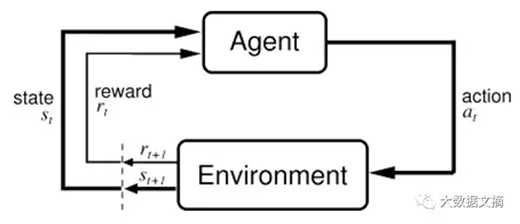
\includegraphics[width=0.6\textwidth]{强化学习过程}
\caption{强化学习的交互过程}
\label{fig:强化学习过程}
\end{figure}

(1)Agent感知当前的环境状态(state);

(2)根据当前的状态和奖赏值(reward),Agent会选择一个行为(action)并执行该行为;

(3)当Agent选择的行为作用于环境时,环境会转移到新的状态,并给出新的奖赏;

(4)Agent根据环境反馈的奖赏,计算回报值(return),并将回报值作为内部更新策略的依据。

 在这一过程中,Agent并不会被告知应该采取哪个行为,而只能经过不断的尝试后,根据得到的环境反馈信息做出判断。Agent选择行为的原则是:所选择的行为应该在以后的学习过程受到环境奖励的概率增大,受到惩罚的概率减小,也就是说,当前采取的行为和最终的目标有关。因为奖励信号是有延迟的,所以Agent有时候宁愿牺牲即时(短期)的奖励以获取更多的长期奖励。因此,试错搜索和延迟回报是强化学习中最重要的两个特征。

 从以上的描述中,可以看出,与监督学习不同,强化学习并不需要多样化的标签数据,而只需要带有回报的交互数据;另外,监督学习是一种反馈学习,即将模型的输出与标签之间所产生的误差信号反馈给模型来指导学习,而在强化学习中,由环境产生的奖赏信号是对所产生行为好坏的一种评价,Agent在行为与评价中获取知识,不断的改进行为方案以适应环境,并不是告诉Agent如何去产生正确的动作。


\section{强化学习的组成要素}
% 介绍马尔科夫决策过程,策略、累计回报、值函数、贝尔曼方程、最优值函数
\paragraph{马尔科夫决策过程}
强化学习可以使用马尔科夫决策过程框架来形式化的描述,MDP通常表示为一个四元组$<S,A,f,h>$,其中:$S$表示有限的状态空间,定义为一个有穷集合$\{ S_1,S_2,\cdots ,S_N \}$,$N$为状态空间的大小。$A$表示有限的行为空间,定义为一个有穷集合$\{ A_1,A_2,\cdots ,A_M \}$,$M$为行为空间的大小。$f$表示状态转移函数,$h$表示奖赏函数。

在马尔科夫决策过程中,考虑在任意的离散时间点$t$时,环境的状态为$S_{t}$,此刻Agent若采取行为$A_t$,就会得到有限的即时奖赏$R_{t}$,并且状态也会相应的转移到下一状态$S_{t+1}$。其中,奖赏$R_{t}$是根据奖赏函数$h$得到的,下一时刻的状态$S_{t+1}$是根据状态转移函数$f$得到的。另外,根据状态转移的情况,可以分为确定性状态转移和随机性状态转移。在确定性状态转移中,状态会转移到确定性的下一状态,而在随机性状态转移中,转移到的下一状态是不确定的,是一个随机变量。

% 又因为马尔科夫决策过程的状态具有马尔科夫性,因此状态转移函数和奖赏函数都仅和当前状态和行为有关,与历史的状态序列和行为序列无关。即:$p(s^{'},r|s,a) = Pr\{S_{t}=s^{'}, R_t=r|S_{t-1}=s, A_{t-1}=a\}$且$\sum_{s^{'}\in S}p(s^{'}|s,a)=1$,$\forall s\in S,\forall a\in A$。
\paragraph{策略和回报}
% \subparagraph{策略}
% 强化学习的目标是从给定的马尔科夫决策过程中,寻找最优的策略。
所谓策略是一个从状态到动作的映射,通常用符号$\pi$表示。
% 指在某一状态下,所采取的动作或所采取动作的概率,。
同样,策略也分为确定性策略和随机性策略,其中确定性策略定义为:$\pi$: $S \to A$ 输出的是一个动作序列,而随机性策略定义为:$\pi$: $S \times A \in [0,1]$ 输出的是该状态下所采取动作的概率:$\pi(s,a)=p[A_{t}=a|S_{t}=s]$。

% \subparagraph{回报}
强化学习的任务是从与环境的不断交互中,学习一个策略$\pi$,使其产生的累积奖赏(cumulative reward)最大化(即回报)。
% 当给定一个策略$\pi$时,如何进行策略的评估呢?此时便用到了累积奖赏的概念。
假设在时刻$t$后接收到的奖赏序列为$\{R_{t+1}, R_{t+2},\cdots\}$,那么采用折扣累积奖赏的方式计算回报可以表示为:
\begin{equation}\label{seq:reward}
G_{t}=\sum_{k=0}^{\infty}\gamma^{k}R_{t+k+1}
\end{equation}

式中,$G_{t}$为回报,$\gamma<1$,为一个常量,称为折扣因子。特别地,在系统与环境的交互过程中,如果任务可以自然地被分为带有终止时间片的片段,则该任务称为情节式(episodes)任务。如果任务无法分解成若干片段,整个任务需要不断的进行下去,则改任务称为连续式(continous)任务。

\paragraph{值函数}
当给定策略$\pi$时,在Agent的学习过程中,考虑评价某一状态的价值,很自然的想法是利用回报来衡量。但是,因为某一状态下的状态序列有很多,所以回报$G_{t}$是个随机变量,不是一个确定的值,无法作为目标函数进行优化。然而,其期望是个确定值,因此可以作为状态值函数的定义:当Agent采取策略$\pi$时,回报服从一个分布,将状态$s$的回报期望值定义为状态$s$的值函数。公式化为:
\begin{equation}
\label{seq2_vs}
v_{\pi}(s)=\mathbb{E}_{\pi}[G_{t}|S_t=s]=\mathbb{E}_{\pi}[\sum_{k=0}^{\infty}\gamma^{k}R_{t+k+1}|S_t=s]
\end{equation}

% Q函数是另一种评估值函数的方法。Watkins指出:。

在某些时候,记录状态行为对的值比只记录状态的值更有用。所以,状态行为值函数定义为在状态$s$下采取行为$a$的回报期望值,公式化为:
\begin{equation}
\label{seq2_qsa}
q_{\pi}(s,a)=\mathbb{E}_{\pi}[G_{t}|S_t=s,A_t=a]
=\mathbb{E}_{\pi}[\sum_{k=0}^{\infty}\gamma^{k}R_{t+k+1}|S_t=s,A_t=a]
\end{equation}

因为上述状态值函数\eqref{seq2_vs}的表达形式在实际应用中很不方便,因此,我们可以经过进一步的推导,得到状态值函数的贝尔曼方程:
\begin{equation}
\label{seq1}
\begin{aligned}
v_{\pi}(s)&=\mathbb{E}_{\pi}[G_{t}|S_t=s]\\
&=\mathbb{E}_{\pi}[R_{t+1}+\gamma G_{t+1}|S_t=s]\\
&=\sum_{a}\pi(a|s)\sum_{s^{'}}\sum_{r}p(s^{'},r|s,a)[r + \gamma\mathbb{E}_{\pi}[G_{t+1}|S_{t+1}=s^{'}]]\\
&=\sum_{a}\pi(a|s)\sum_{s^{'},r}p(s^{'},r|s,a)[r+\gamma v_{\pi}(s^{'})], \forall s \in S
\end{aligned}
\end{equation}
其中,$p(s^{'},r|s,a) = Pr\{S_{t+1}=s^{'}, R_{t+1}=r|S_{t}=s, A_{t}=a\}$,表示在状态$s$时执行行为$a$下,转移到下一个状态$s_{'}$并且得到奖赏$r$的概率。

同样地,也可以得到状态行为值函数的贝尔曼方程:
\begin{equation}
\label{seq2}
\begin{aligned}
q_{\pi}(s,a)=\sum_{s^{'},r}p(s^{'},r|s,a)[r+\gamma \sum_{a'}\pi(a'|s') q_{\pi}(s^{'},a^{'})], \forall s \in S, \forall a \in A
\end{aligned}
\end{equation}

计算值函数的目的是为了构建学习算法从数据中学习到最优策略,而每个策略对应着一个状态值函数,那么最优策略自然对应着最优状态值函数。所谓的最优状态值函数$v_{*}(s)$是指所有策略中值最大的值函数,即$v_{*}(s)==\max_{\pi}v_{\pi}(s)$,同样地,最优状态行为值函数$q_{*}(s,a)$为在所有策略中值最大的状态行为值函数,即$q_{*}(s,a)=\max_{\pi}q_{\pi}(s,a)$

因此,我们又可以由式\eqref{seq1}和式\eqref{seq2}进行推导(因为篇幅限制,推导过程略),分别得到最优状态值函数和最优状态行为值函数的贝尔曼最优方程:
\begin{equation}
\begin{aligned}
v_{*}(s)=\max_{a}\sum_{s^{'},r}p(s^{'},r|s,a)[r+\gamma v_{\pi}(s^{'})]
\end{aligned}
\end{equation}
\begin{equation}
\begin{aligned}
q_{*}(s,a)=\sum_{s^{'},r}p(s^{'},r|s,a)[r+\gamma \max_{a'} q_{\pi}(s^{'},a^{'})]
\end{aligned}
\end{equation}

最后,若求出了最优状态行为值函数,最优策略可以通过直接最大化 $q_{*}(s,a)$来决定:
\begin{equation}
\begin{aligned}
\pi_{*}(a|s) = 
    \begin{cases}
        1 & if \ a=\argmax_{a\in A}{q^{*}(s,a)},\\
        0 & otherwise.
    \end{cases}
\end{aligned}
\end{equation}

最后,需要强调的是:从公式\eqref{seq2_vs}和公式\eqref{seq2_qsa}可以看出,值函数是对未来奖赏的一种预测,对于一个状态$s$,如果它的奖赏很低,但并不意味着它的状态值就低,因为如果状态$s$的后续状态产生较高的奖赏,仍然可能得到比较高的状态值,这就是本文将强化学习技术用于求解营销问题,进而获取长期收益最大化的主要原因。但是,确定值函数需要Agent在其整个生命周期内通过一系列的观察,不断的估计才能得到。所以,我们接下来要做的就是如何快速而准确的获取值函数。

\section{强化学习经典算法}
根据是否依赖于环境,强化学习的求解方法可以分为基于模型的动态规划法和模型无关的强化学习算法。在基于模型的动态规划法中,需要提供精确的环境模型,然后根据环境的动态性利用贝尔曼方程迭代的求解值函数,其本质是动态规划(Dynamic Programming, DP)的思想,通过不断迭代直至稳定,得到精确解。模型无关的强化学习算法无需提供环境模型,根据agent与环境的不断交互收集样本,然后直接利用样本求解状态值函数和状态行为值函数。主要包括蒙特卡罗(Monte Carlo, MC)法和时间差分(Temporal Difference, TD)等算法。

\subsection{动态规划法}
动态规划法是指在给定模型的情况下,求解最优策略的方法。主要包括策略迭代和值迭代两种方法。

策略迭代算法包括策略评估和策略改善两个步骤,且两个步骤交替进行。在策略评估中,算法的每次迭代是建立在上一轮策略改善的基础上,对状态空间中的每个状态进行扫描,并利用贝尔曼方程进行更新,经过不断的迭代,值函数最终收敛至不动点。在策略改善中,算法利用上一轮策略评估得到的值函数,以贪心的方式生成一个新的策略。两
个过程不断交替,直至策略收敛至最终策略。特别地,贝尔曼方程$\eqref{seq1}$中状态值函数$v_{\pi}(s)$使用了其后继状态的值函数$v_{\pi}(s^{'})$来表示,这是自举(bootstrapping)的思想。

以行为状态值函数的策略迭代过程为例,:
\begin{displaymath}
\begin{aligned}
\pi_{0}\xrightarrow{E}q_{\pi_0}\xrightarrow{I}\pi_{1}\xrightarrow{E}q_{\pi_1}\xrightarrow{I}\pi_{2}\xrightarrow{E}q_{\pi_2}\xrightarrow{I}\pi_{3}\xrightarrow{E} \cdots \xrightarrow{I}\pi_{*}\xrightarrow{E}q_{\pi_{*}}
\end{aligned}
\end{displaymath}
其中$E$代表策略评估过程,$I$代表策略改善过程。初始时,策略和值函数都是随机的。在策略评估时,针对每一个状态行为值,使用贝尔曼方程$\eqref{seq2}$进行值函数的更新,直到$q_{k+1}$稳定便结束本轮迭代:
\begin{equation}
\begin{aligned}
q_{k+1}(s,a)=\sum_{s^{'},r}p(s^{'},r|s,a)[r+\gamma \sum_{a'}\pi(a^{'}|s^{'}) q_{k}(s^{'},a^{'})]
\end{aligned}
\end{equation}
在策略改善时,对所有的状态,使用贪婪方法求出新的策略:
\begin{equation}
\begin{aligned}
\pi_{k+1}(s)=\argmax_{a}q_{k+1}(s,a)
\end{aligned}
\end{equation}
在收敛到最优策略时,每一轮的策略都好于前一轮的策略。当策略$\pi$稳定时,迭代过程结束,即得到最优值函数$q_{*}(s,a)$和最优策略$\pi_{*}$。

值迭代算法是对策略迭代的简化,也包括策略评估和策略改善两个环节。与策略迭代不同的是,它不需要等到在策略评估值函数完全收敛时才进行下一次的迭代,而是对全部的状态行为空间每进行一次扫描(更新)就进行策略改善,加快了值函数的收敛速度。对每一个状态行为对,值迭代的更新公式如下:
\begin{equation}
\begin{aligned}
q_{k+1}(s,a)=\sum_{s^{'},r}p(s^{'},r|s,a)[r+\gamma \max_{a^{'}} q_{k}(s^{'},a^{'})]
\end{aligned}
\end{equation}
直到$q_{k+1}$稳定,算法结束。此时因为值函数已经收敛,直接对值函数使用贪心方法就可以得到最优策略。

\subsection{蒙特卡洛方法}
在求解强化学习问题时,由于动态规划法需要提供完整的环境模型且计算代价太大,限制了其在实际场景中的应用。当没有环境模型时,我们可以采用蒙特卡罗方法计算值函数,即用经验平均的思想代替随机变量的思想。其中,经验是指按照该策略做了很多次试验,产生很多情节(episode),每一个情节就是一次实验,平均就是指的平均值,按照求解方法不同又可以分为第一次访问(first-visit)蒙特卡罗方法和每次访问(every-visit)蒙特卡罗方法。在与环境的交互过程中,当一个情节结束后,则进行值函数的更新和策略的改善。另外,值函数的更新可采取可递增(Incremental )计算均值的方法,公式为:
\begin{equation}
\begin{aligned}
V_{k+1}(s)=V_{k}(s)+ \alpha(G_{t}-V_{k}(s))
\end{aligned}
\end{equation}
其中,$\alpha$为学习率,$G_{t}$为从状态$s$出发至情节结束所获的的累积折扣奖赏。

在动态规划中,为了保证值函数的收敛,算法会扫描状态空间的每一个状态。而蒙特卡罗方法想要充分评估值函数的前提是保证每个状态都可以被访问到,因此MC采用了探索性初始化(Exploring Start)的方法,即在每一个情节在迭代时,其初始状态都是随机分配的。

\subsection{时间差分方法}
相比于动态规划法,蒙特卡罗法使用了经验平均,虽然摆脱了对模型的依赖,但是不需要等到每个情节结束就可以进行值函数评估和策略更新,所以学习速度慢,学习效率不高。而动态规划因为使用了bootstrapping思想,所以可以在情节未结束时就可以根据未来值函数估计当前的值函数。时间差分法综合了两者的优点,融合了蒙特卡罗的采样方法和动态规划的bootstrapping思想。

所谓时间差分是指对同一事件或变量在连续两个时刻观测的偏差。TD(0)算法是指一步更新,即值函数直接根据下一个时间步进行学习,估计下一个状态的值函数。
假设在状态$S_{t}$时,Agent采取行为$A_{t}$,获得奖赏$R_{t}$的同时状态转移到$S_{t+1}$。因为环境从状态$S_{t}$向$S_{t+1}$以外的其它状态转移的概率为0,设$V(S_{t})$为最优$v_{*}(S_{t})$的估计值,那么状态$S_{t}$的值函数为:
\begin{equation}
\begin{aligned}
V(S_{t})=R_{t+1}+\gamma V(S_{t+1})
\end{aligned}
\end{equation}
时刻$t$的时间差分为:
\begin{equation}\label{shijiachafen}
\begin{aligned}
\delta_{t}=R_{t+1}+\gamma V(S_{t+1})-V(S_{t})
\end{aligned}
\end{equation}
那么,值函数的更新公式为:
\begin{equation}
\begin{aligned}
V(S_{t}) \gets V(S_{t})+\alpha (R_{t+1}+\gamma V(S_{t+1})-V(S_{t}))
\end{aligned}
\end{equation}
式中,$\alpha$为步长参数,控制学习率,$R_{t+1}+\gamma V(S_{t+1})$称为TD目标,$\delta_{t}=R_{t+1}+\gamma V(S_{t+1})-V(S_{t})$为TD偏差。

根据探索策略(行为策略)和评估策略是否为一个策略,可以将强化学习方法分为同策略(on-policy)和异策略(off-policy)两种方法。同样,时间差分方法也包括了同策略的Sarsa方法和异策略的Q-learning方法。在Sarsa方法中,行动策略和评估策略都是$\epsilon-greedy$的方法,对应的算法伪代码如$\ref{algo:algorithm_1}$所示。

\begin{algorithm}[htbp]
\small
\SetAlgoLined
\SetKwRepeat{Repeat}{Repeat}{until} 
% \KwData{this text}
% \KwResult{how to write algorithm with \LaTeX2e }
初始化$Q(s,a)$,$\forall s \in S$,$\forall a \in A$, 给定参数$\alpha$,$\gamma$\;
\Repeat{所有的$Q(s,a)$收敛}{
初始化起始状态$s$\;
根据$\epsilon-greedy$策略在状态$s$下选择行为$a$\;
\Repeat((对每个情节的每一步)){$s$是终止状态}{
	在状态$s$下选择行为$a$,得到奖赏$r$和下一个状态$s^{'}$\;
	在状态$s^{'}$下根据$\epsilon-greedy$策略得到动作$a^{'}$\;
	$Q(s,a) \gets Q(s,a)+\alpha[r+\gamma Q(s^{'},a^{'}) - Q(s,a)]$\;
	$s=s^{'}$,$a=a^{'}$\;
	}
}
输出最终策略:$\pi(s)=\argmax_{a}Q(s,a)$\;
\caption{Sarsa算法}
\label{algo:algorithm_1}
\end{algorithm}

与Sarsa方法不同,在Q-learning中,行为策略采用$\epsilon-greedy$策略,而目标策略采用贪婪策略,故又称为异策略Q-learning算法,其伪代码如$\ref{algo:algorithm_2}$所示。
\begin{algorithm}[htbp]
\small
\SetAlgoLined
\SetKwRepeat{Repeat}{repeat}{until} 
% \SetAlgoRefName{algorithm_2}
初始化$Q(s,a)$,$\forall s \in S$,$\forall a \in A$, 给定参数$\alpha$,$\gamma$\;
\Repeat{所有的$Q(s,a)$收敛}{
初始化起始状态$s$\;
% 根据$\epsilon-greedy$策略在状态$s$下选择行为$a$\;
\Repeat((对每个情节的每一步)){$s$是终止状态}{
	在Q函数中,根据$\epsilon-greedy$策略在状态$s$下选择行为$a$\;
	执行行为$a$后,得到回报$r$和下一状态$s^{'}$\;
	$Q(s,a) \gets Q(s,a)+\alpha[r+\gamma \max_{a} Q(s^{'},a)-Q(s,a)]$\;
	$s=s^{'}$\;
	}
}
输出最终策略:$\pi(s)=\argmax_{a}Q(s,a)$\;
\caption{Qlearning算法}
\label{algo:algorithm_2}
\end{algorithm}

在TD(0)中,更新当前值函数时,只用到了下一步状态值函数。而TD($\lambda$)考虑从未来的多步进行学习,并且采用加权的方法融合这多步的估计值,$\lambda \in [0,1]$决定了向未来观察的时间步长度。即
\begin{equation}
\begin{aligned}
V(S_{t} )\gets V(S_{t})+\alpha (G^{(\lambda)}_{t}-V(S_{t}))
\end{aligned}
\end{equation}
其中,
\begin{displaymath}
\begin{aligned}
G^{(\lambda)}_{t}=(1-\lambda) \sum_{n=1}^{\infty} \lambda^{n-1} G^{(n)}_{t}\\
\end{aligned}
\end{displaymath}
\begin{displaymath}
\begin{aligned}
G^{(n)}_{t}=R_{t+1}+\gamma R_{t+1}+ \cdots +\gamma^{n-1} R_{t+n}+\gamma^{n} V(S_{t+n})
\end{aligned}
\end{displaymath}

这就是TD($\lambda$)的前向视角表达形式,但是,这种方式需要等到整个实验结束才能计算。后向视角利用增量式的更新方式,不需要等到实验结束就可以更新当前状态的值函数,并且引入了资格迹$Z_{t}(s)$的概念,资格迹记录了最近被访问过的状态,也就是说,最近且最频繁被访问到的状态会被赋予最大的“资格”。更新方式为:

(1)首先,计算当前状态的TD偏差:$\delta_{t}=R_{t+1}+\gamma V(S_{t+1})-V(S_{t})$

(2)其次,更新资格迹:$Z_{t}(s) = 
    \begin{cases}
        \gamma \lambda Z_{t-1} & if s \neq s_{t},\\
        \gamma \lambda Z_{t-1}+1 & if s = s_{t}.
    \end{cases}$

(3)最后,对状态空间中的每个状态$s$,更新值函数:$V(s) \gets V(s)+\alpha \delta_{t} Z_{t}(s)$

综上,后向视角的时间差分方法不仅不需要环境模型,而且利用了增量在线的机制,实现方式简单有效,同时也保证了策略的实时性,被认为是强化学习中最核心的算法。

\section{值函数逼近方法}
至此,我们可以归纳出基于值函数的强化学习的基本步骤是:先评估值函数,然后再利用值函数改善当前的策略。其中,值函数的评估是关键。

在之前所介绍的强化学习方法中,值函数其实是一个表格,其索引是状态或者状态行为对,值迭代更新实际上就是这张表格的迭代更新,因此,这种强化学习称为表格型强化学习,它有一个前提条件:状态空间和行为空间都是离散的,并且状态空间和行为空间不能太大。然而,现实中的很多问题都具有很大的状态(行为)空间,甚至是连续的状态(行为)空间,比如围棋有 $10^{170}$  个状态空间,控制直升机飞行需要的是一个连续的状态空间。在这种情况下,需要我们利用函数逼近的方法表示值函数。从数学的角度来看,函数逼近方法可以分为参数化函数逼近和非参数化函数逼近,其中参数化函数逼近又分为线性参数逼近和非线性参数逼近。

\subsection{参数化函数逼近}
参数化函数逼近是从参数空间到值函数空间的映射,函数的形式和参数的个数事先由先验知识预设,而且参数是通过与目标函数有关样本数据来调整的。对于状态(状态行为)值函数可以由一组参数$\bm{\theta}\in \mathbb{R}^{n} $ 来近似,即:
\begin{equation}
\label{seq_2_3_2}
\begin{aligned}
&\hat{v}(s;\bm{\theta})\approx v_{\pi}(s)\\
&\hat{q}(s,a;\bm{\theta})\approx q_{\pi}(s,a)
\end{aligned}
\end{equation}

我们可以发现,在近似的状态值函数$\hat{v}(s;\bm{\theta})$中,针对每个状态,不再存储其状态值,而是只存储一组参数。把从已知的状态中到的值函数,推广至那些未碰及的状态中,这对于拥有大规模的状态空间来说,相当于对其状态空间进行了压缩。由于 $\bm{\theta}\in \mathbb{R}^{n}$,因此所需的存储开销为$O(n)$,当状态空间规模较大且均为离散时,$n$远远小于为每个状态存储值的开销$|S|$。

以状态值函数为例,我们可以得到目标函数为:
\begin{equation}
\label{seq:fun_approxi_obj}
\begin{aligned}
\argmin_{\bm{\theta}}(v_{\pi}(s)-\hat{v}(s;\bm{\theta}))^2
\end{aligned}
\end{equation}

即通过寻找参数向量$\bm{\theta}$,最小化近似函数$\hat{v}(s;\bm{\theta})$与真实函数$v_{\pi}(s)$的均方差。

值函数更新可以分为增量式学习方法和批学习方法。其中,随机梯度下降法是最常用的增量式学习方法。

由公式$\eqref{seq:fun_approxi_obj}$,我们可以得到参数的随机梯度更新公式为:
\begin{equation}
\begin{aligned}
\bm{\theta} \gets \bm{\theta}+\alpha[v_{\pi}(s)-\hat{v}(S_{t};\bm{\theta})]\triangledown_{\theta} \hat{v}(S_{t};\bm{\theta})
\end{aligned}
\end{equation}

进而,得到值函数的更新如下:
\begin{equation}
\label{seq:gradient}
\begin{aligned}
\triangle \bm{\theta} = \alpha (v_{\pi}(s)-\hat{v}(s;\bm{\theta})) \triangledown_{\theta} \hat{v}(s;\bm
{\theta})
\end{aligned}
\end{equation}

然而,公式$\eqref{seq:gradient}$并不能直接用于强化学习中,因为公式里有一个真实价值函数$v_{\pi}(s)$,或者是一个具体的数值,而强化学习没有监督数据。

从表格型值函数的更新过程中,我们可以看出无论是蒙特卡罗方法还是时间差分方法,都是朝着一个目标值更新的,这个目标值在蒙特卡罗方法中是$G_{t}$,在时间差分方法中是$R_{t+1}+\gamma Q(S_{t+1},A_{t+1})$,在$TD(\lambda)$中是$G^{\lambda}_{t}$。所以,如果将表格型值函数的更新过程推广至值函数逼近过程,那么,逼近值函数$\hat{v}(s;\bm{\theta})$的过程实际上可以看作是一个监督学习的过程,其数据和标签对为$<S_{t}, v_{\pi}(S_{t})>$,其中$v_{\pi}(S_{t})$等价于蒙特卡罗方法中的$G_{t}$,时间差分方法中的$R_{t+1}+\gamma Q(S_{t+1},A_{t+1})$,以及$TD(\lambda)$中是$G^{\lambda}_{t}$。因此,只要将公式$\eqref{seq:gradient}$总的$v_{\pi}(S_{t})$做相应替换就可以进行求解了。

在增量式学习方法学习方法中,每次更新模型需要与环境交互,数据使用一次即抛弃,导致样本使用效率不高。而所谓批方法是从给定一段时期的经验中抽取数据集:$D={<S_{1},v^{\pi}_{1}>,<S_{2},v^{\pi}_{2}>,\cdots,<S_{T},v^{\pi}_{T}>}$中,找到最好的拟合函数$\hat{v}(s;\bm{\theta})$,使的$LS(\bm{\theta})=\sum_{t=1}^{T}(v^{\pi}_{t}-\hat{v}^{\pi}_{t}(S_{t},\bm{\theta}))^2$ 最小,这种方法相当于经历重现(Experience Replay),把一段时期内的经历重新过一遍,更新参数,因此样本的利用效率高。

参数化函数逼近根据所使用逼近函数的不同,可分为参数化线性函数逼近和参数化非线性函数逼近两种。

以状态值函数为例,线性函数逼近可以表示为:
\begin{equation}
\begin{aligned}
\hat{v}(s;\bm{\theta})=\sum^{n}_{i=1}\phi_{i}(s) \bm{\theta}_{i}=\bm{\theta }^{T} \bm{\phi}(s)
\end{aligned}
\end{equation}
其中,$\bm{\theta}=(\bm{\theta}_{1},\cdots,\bm{\theta}_{n}) \in \mathbb{R}$,$\bm{\phi}(s)=(\phi_{1}(s),\cdots,\phi_{n}(s))^{T}$为状态$s$的特征向量,$\phi_{i}(s)$称为特征函数或者称为基函数,常见的基函数有:多项式基函数、傅立叶基函数以及径向基函数等。线性函数逼近不但形式简单、而且可以收敛到全局最优,缺点是表征能力较弱,而且基函数的形式需要事先选定,这也限制了函数的逼近能力。
% 但是正是由于其具备良好的收敛性和理论简单性,在强化学习的参数化方法中得到了充分应用。

在非线性函数逼近中,函数逼近器是关于参数$\bm{\theta}$的非线性函数。到在强化学习的应用场景中,一个状态数据是可能是持续流入的,而且下一个状态通常与前一个状态是高度相关的。因此,我们需要一个适用于非静态、非独立均匀分布的数据的训练方法来得到近似函数。在众多的非线性方法中,神经网络是最为符合的,因为它关于状态可导而且是迭代求解的。

神经网络可以看成是一种参数化基函数的方法。由于基函数的参数是从数据中学习得到的,因此其表示能力大大提升,神经网络的每层都可看成是基于上一层的新的基函数,也就是特征。从这个意义上说,后面一层是前面一层的抽象,这样可以对高维输入降维。

所以,和线性逼近器相比,非线性函数逼近的优点是有很强的表征能力和逼近能力,可以对目标函数以任意精度逼近,但是其收敛性难以保证,容易陷入局部最优,使的学术界对其的研究停滞了很长时间,直到2013年,DeepMind团队提出了一些改进的深度强化学习的训练方法,很大程度上解决了神经网络在强化学习问题中的收敛性问题,并且取得了令人振奋的实验表现,引发了针对此问题的新的研究热潮。具体细节可以参见本文第三章关于DQN的介绍。

\subsection{非参数化函数逼近}
在参数化函数逼近过程中,基函数的形式和参数的个数都需要提前设定,并且值函数的逼近效果很大程度上受到人为的经验的影响。而在非参数化函数逼近中,参数的个数以及基函数的形式并不是固定的,而是由样本决定,具有很高的灵活性。非参数化函数逼近方法包括基于核函数的方法和基于高斯过程的方法。因为本文第四章是使用的基于核函数的非参数化函数逼近的方法,所以此处仅对基于核的非参数函数逼近进行介绍。

基于核函数逼近模型可以表示为
\begin{equation}
\begin{aligned}
&\hat{q}(s,a;\bm{\theta})=\sum^{n}_{i=1}\bm{k}((s,a),(s_{i},a_{i}))\bm{\theta}_{i}\\
&\hat{v}(s;\bm{\theta})=\sum^{n}_{i=1}\bm{k}((s),(s_{i}))\bm{\theta}_{i}
\end{aligned}
\end{equation}
式中,$\bm{\theta}_{1},\cdots,\bm{\theta}_{n}$为参数向量,$\{(s_{i},a_{i})|i=1,\cdots,n\}$为样本集合,$\bm{k}:S\times A \times S \times A \to \mathbb{R} $为核函数。其中,常用的核函数有线性核函数、多项式核函数、径向基核函数以及Sigmoid核函数等。

利用核函数法逼近值函数的关键是能够将问题构造成一个带有核函数的优化问题。非参数化函数学习过程中完全依赖于样本,虽然带来一定的逼近灵活性,但是收敛性难以得到保证。

\section{本章小结}
 本章主要介绍了强化学习的相关理论基础知识。首先,对强化学习的整体交互过程进行简单介绍,让读者可以对强化学习有一个直观的认识和体会;接着,介绍了强化学习的框架马尔科夫决策过程以及强化学习的三个要素:策略、回报和值函数;然后,介绍了强化学习基于模型和模型无关的三种求解方法;最后,针对大规模问题,介绍了求解值函数的两种逼近方法:参数化函数逼近以及非参数化函数逼近。为后面章节做了铺垫。
\chapter{基于RNN的深度强化学习混合模型在直复营销场景中的建模}
% 首先介绍直复营销问题使用强化学习研究的现状(函数逼近存在的问题,以及现行的解决方案和思路,从而引出本文的方法思路)
% 介绍深度强化学习
% 介绍本文提出的混合网络模型算法
在直复营销的场景中,企业以追求客户的生命周期价值最大化为目标,这与强化学习以追求累计奖赏最大的目标不谋而合。另外,在该场景中企业需要与顾客不断的进行营销行为,因此属于序列决策问题,并且因为场景的复杂性,还存在用户状态部分可观测的问题。而以RNN为代表的循环神经网络正巧可以在很好的处理序列问题的基础上,还可以利用神经网络自动的学习隐藏状态的表达方式。所以,结合以上两点,本章提出了基于RNN的深度强化学习的混合模型。在该模型中,使用RNN网络来学习和提高针对隐藏状态的表征能力,然后利用DQN网络来逼近Q值函数,充分利用了两个模型的优点。另外,为了提高训练时收敛的速度和精度,提出了两种改进的混合模型网络:一步混合模型1-RNN+DQN和两步混合模型2-RNN+DQN。

\section{直复营销问题概述}
直复营销是客户关系管理中的一项重要议题。它是通过企业长时间的与客户进行营销交互,并且结合所采取的营销行为和客户的响应情况进行分析,
以此来判断客户的对营销产品的喜好,进而可以辅助企业进行之后的营销决策。具体来说,在每个需要进行营销的时刻点,企业会对客户采取营销行为,比如发送宣传单、促销邮件或者优惠券等等,作为反馈,客户可能会访问该企业的相关资讯或者会完成一定金额的订单又或者会简单的忽略掉此次的营销行为。所以,企业需要在进行营销活动的时候做出对哪些客户进行营销的决策,以使的企业产生的收益最大化。

在直复营销场景中,我们需要注意的是,假如企业在某一时刻对某一客户采取了营销行为,客户可能会即刻给出反馈,也能会过了很长时间才会产生反馈信息。也就是说,营销行为对用户的影响是长期的而且用户对营销行为的反应是存在延迟的。所以,企业通常把最大化用户生命周期价值(Life-Time Value, LTV)作为评价营销效果的重要指标\citep{dwyer1997customer}。通过前面的介绍,我们知道强化学习在学习过程中考虑了延迟奖赏,并且以追求长期回报最大化为目标,所以直复营销问题就可以自然的表述为一个基本的强化学习问题,其中,即时利润看作是奖赏,LTV作为长期的价值函数。文献\citep{tkachenko2015autonomous,pednault2002sequential,silver2013concurrent}都正是以此想法为出发点,将强化学习技术应用在广告营销中,并且取得了较好的表现。

然而,与机器人和人机交互等现实应用场景中所面临的问题类似,在直复营销场景中,客户的状态(马尔科夫状态)是部分可观测的,这影响了强化学习技术在这些场景中的表现。根据马尔科夫性我们可以知道,客户的当前状态可以完全概括了他与企业在此之前的整个交互历史,也就是说客户的未来响应情况与之前的交互历史无关,只与在当前状态和未来的行为有关。然而,在直复营销这种复杂的现实场景中,构建这种具有马尔科夫性的状态是很难的。即使像在直复营销中比较常用的Recency-Frequency-Monetary用户价值模型\citep{tkachenko2015autonomous},也仅仅捕获到了客户真实状态中的部分信息。因此,对这些场景使用强化学习之前,进行隐藏状态的推断表示是很重要的。

在强化学习的研究和应用中,处理部分可观测状态最常用的方法就是使用部分可观测的马尔科夫决策过程(Partially Observable Markov  Decision Process,POMDP)\citep{kaelbling1998planning},并且已经在一些诸如机器人、人机对话等领域取得了不错的表现\citep{pineau2003point,williams2007partially}。在POMDP中,因为agent对环境观测的局限性,所以多了一步agent对当前所处状态可信度的判断,
但是对当前状态可信度的判断需要借助领域专家自定义的隐状态,而这些领域知识在一些复杂的现实应用中是很难获得的。

近年来,深度强化学习成功的应用在了游戏、围棋等领域。它们主要是将强化学习技术和深度神经网络相结合,其中,利用神经网络在逼近价值函数的同时也可以推断出环境的隐含状态表示方法。与POMDP不同的是,深度神经网络在不依靠专家领域知识的前提下,对任何给定的问题都可以自动的给出隐藏状态的合理表示方法\citep{deng2014deep},从而解决了在设计隐状态时所面临的困扰。以上本文选择使用深度强化学习解决直复营销问题的出发点,特别的,我们对现有的网络结构做了近一步的改进优化。

\section{深度强化学习DQN}
\subsection{Q-learning回顾}
在算法$\ref{algo:algorithm_2}$中,我们对Q-learning算法做了详细介绍,Q-learning方法主要思想是异策略的时间差分方法。

异策略,就是指的行为策略(产生数据的策略)和要评估的策略不是一个策略。在Q-learning中,行为策略是第6行的$\epsilon-greedy$的策略,而用于评估和改善的策略是第7行的贪婪策略(每个状态取值函数最大的那个行为)。

时间差分方法,是指利用时间差分目标来更新当前行为的值函数。在Q-learning中,时间差分的目标就是$r+\gamma \max_{a} Q(s^{'},a^{'})$。
\subsection{DQN}
 深度强化学习以DQN最为代表性,它就是在Q-learning的基础上修改得到的,主要进行了以下三个方面的改进。

 \paragraph{利用卷积神经网络逼近值函数}
 DQN利用深度卷积神经网络逼近值函数。如图\ref{fig:CNN_DQN}所示为状态行为值函数的逼近网络结构。利用神经网络逼近值函数属于参数化的非线性逼近方法,不仅具有很强的表征能力,而且还可以自动的捕捉到环境的隐状态信息。此处的值函数对应着一组参数,也就是神经网络中每层网络的参数,我们可以用向量$\mathbf{\theta}$表示,对应的值函数可以表示为$Q(s,a;\mathbf{\theta})$,所以对值函数的更新也就是对参数向量$\mathbf{\theta}$,当网络结构确定后,$\mathbf{\theta}$就代表着值函数。DQN所使用的网络结构是三个卷基层加两个全连接层。
\begin{figure}[htbp]
\centering
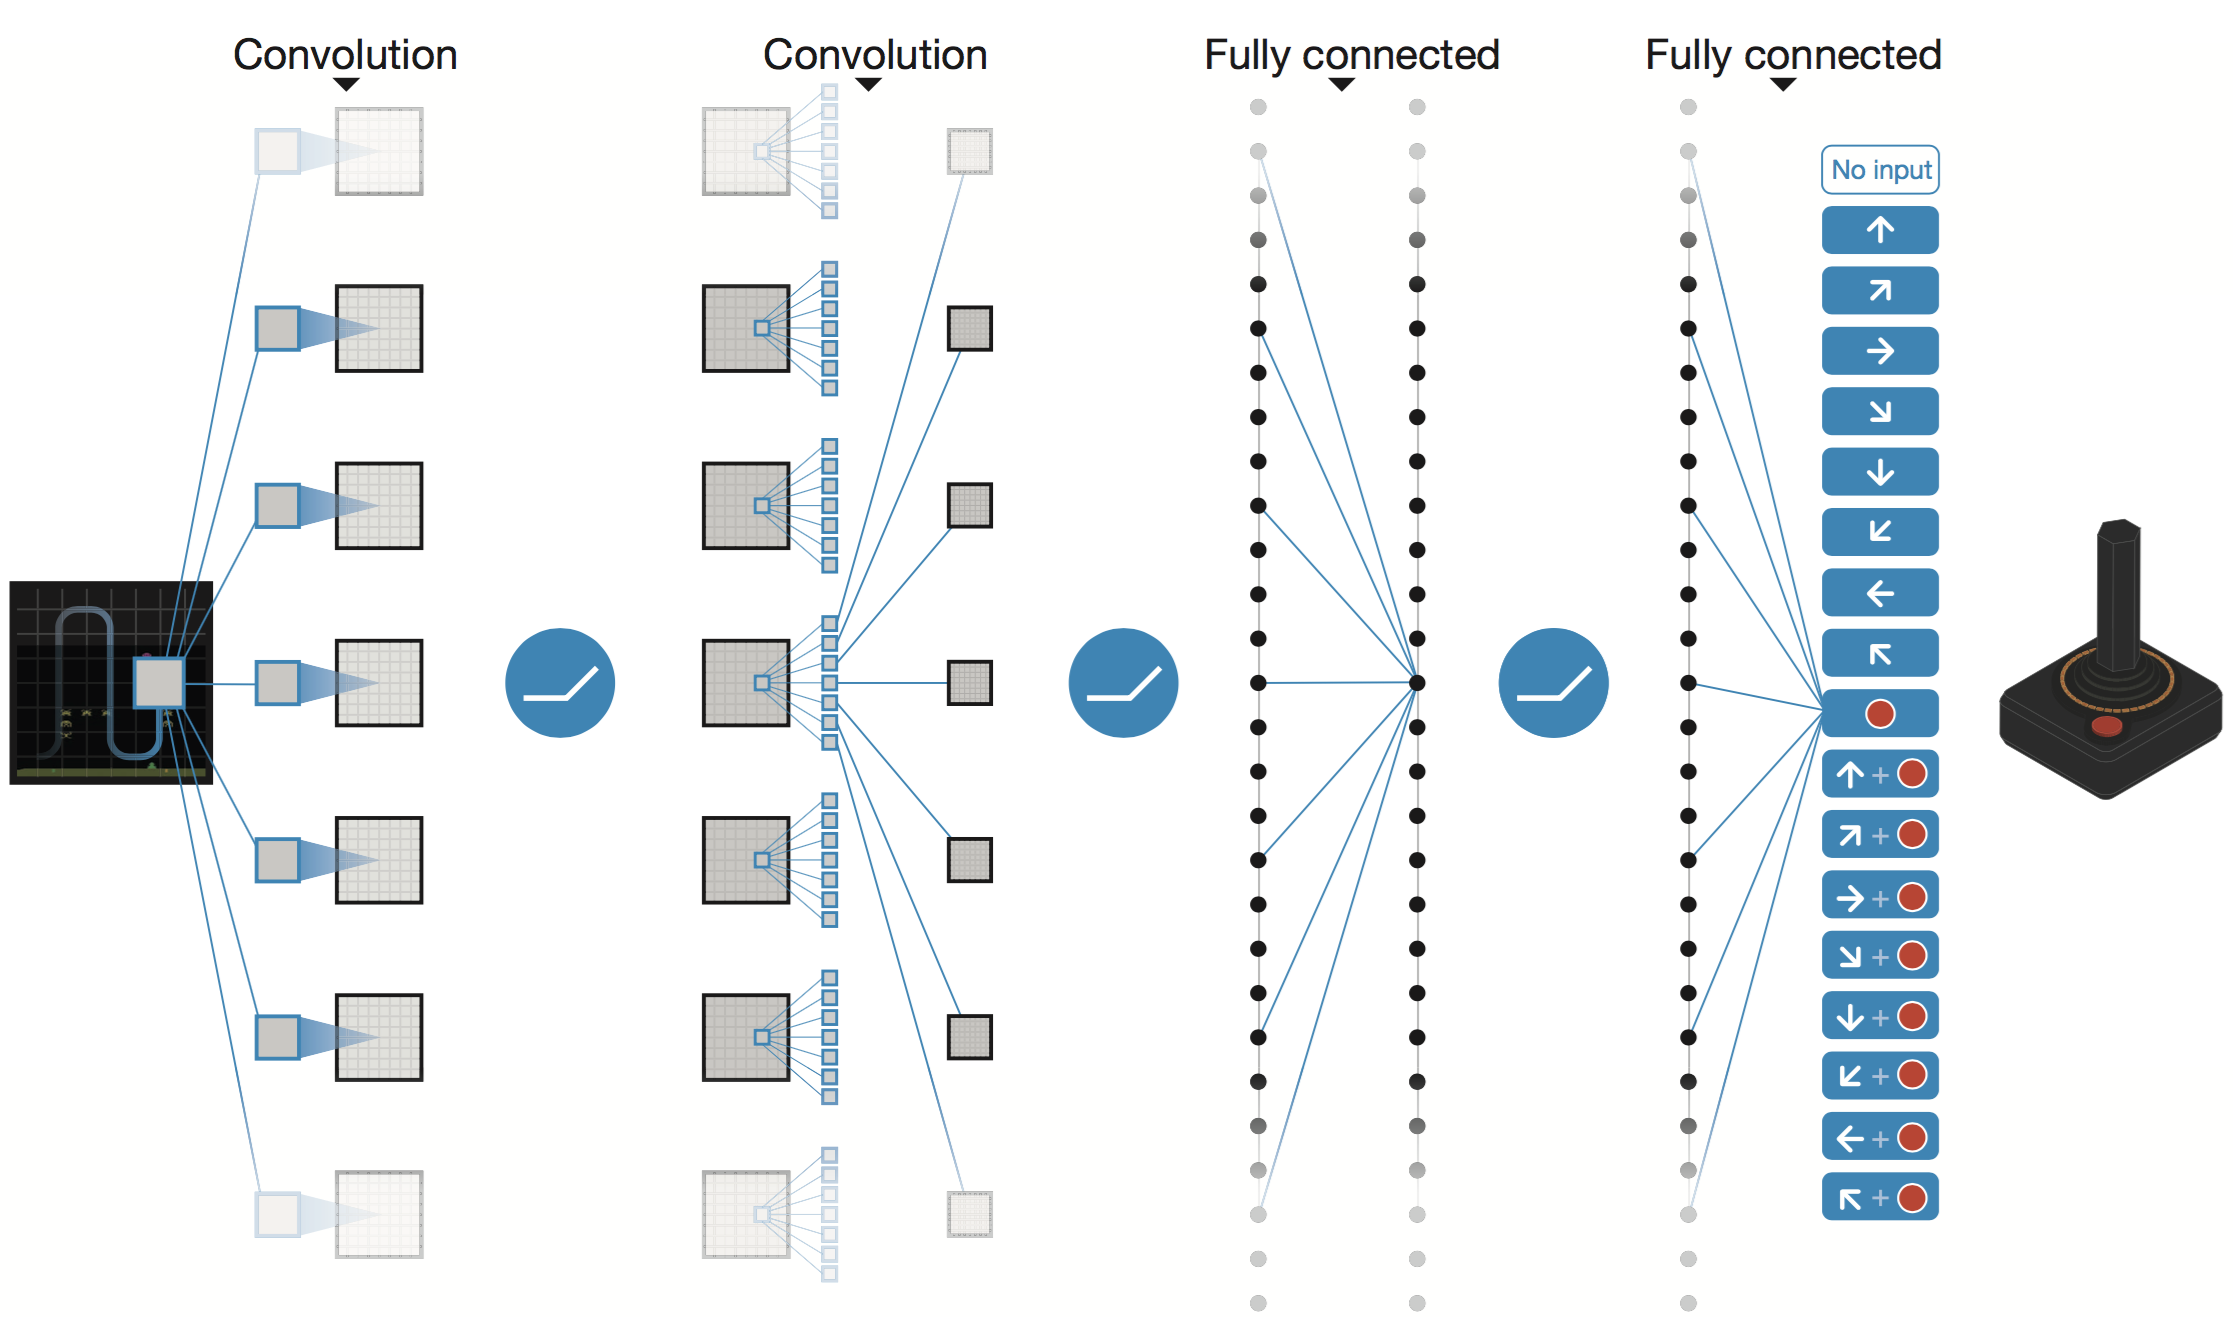
\includegraphics[width=1.0\textwidth]{CNN_DQN}
\caption{DQN状态行为值函数逼近网络}
\label{fig:CNN_DQN}
\end{figure}

其实,1995年Bertsekas等人最早将神经网络应用在在强化学习的值函数逼近中,取得了相比线性逼近较好的结果,但是往往会出现不稳定不收敛的情况\citep{bertsekas1995neuro}。此后,众多学者在这个方向上一直没有突破,直到DeepMind团队的出现。

 \paragraph{设置经验回放机制}
DeepMind团队的创始人Hassabis是神经科学的博士,他主要研究人类大脑中的海马体,海马体是大脑中主要负责记忆和学习的部分。他在研究时发现,人类在睡觉的时候,海马体会把一天的记忆重放给大脑皮层,利用这个启发机制,DeepMind团队的研究人员设计了一种神经网络的训练方法:经验回放。

经验回放是指,在强化学习的过程中,agent将数据存储在一个数据库中,再利用均匀采样的方法从数据库中抽取数据,然后利用抽取的数据训练神经网络。通过这种方法可以使的神经网络训练收敛且稳定。因为在训练神经网络时,我们假设的前提是训练数据是独立同分不的,但是通过强化学习采集的数据之间存在关联性,利用这些数据进行顺序训练,神经网络难免会不稳定。但是利用经验回放可以打破这种数据间的关联性。

 \paragraph{设置独立的目标网络}
与表格型Q-learning强化学习算法不同的是,利用神经网络对值函数进行逼近时,对值函数的更新其实就是对参数向量$\mathbf{\theta}$的更新,其更新方法时梯度下降法,因此算法$\ref{algo:algorithm_2}$第7行值函数的更新实际上变成了进度学习的一次更新过程,其梯度下降法为:
\begin{displaymath}
\begin{aligned}
\mathbf{\theta}_{t+1}=\mathbf{\theta}_{t}+\alpha[r+\gamma \max_{s^{'}}Q(s^{'},a^{'};\mathbf{\theta})-Q(s,a;\mathbf{\theta})]\triangledown Q(s,a;\mathbf{\theta})
\end{aligned}
\end{displaymath}
其中,$r+\gamma \max_{s^{'}}Q(s^{'},a^{'};\mathbf{\theta}$为TD目标,在计算$\max_{s^{'}}Q(s^{'},a^{'};\mathbf{\theta}$时用到的参数向量为$\mathbf{\theta}$。

我们称计算TD目标时所用的网络为TD网络。在DQN算法出现之前,利用神经网络逼近值函数时,计算TD目标的状态行为值函数所用的网络参数$\mathbf{\theta}$,与梯度计算中要逼近的值函数所用的网路参数向量相同,这样就容易导致数据间存在关联性,从而使训练不稳定。为了解决此问题,DeepMind提出计算TD目标的网络参数为$\mathbf{\theta}^{-}$,计算值函数逼近网络表示为$\mathbf{\theta}$;用于状态行为值函数逼近的网络每一步都要更新,而用于计算目标的网络则是每个固定的步骤更新一次。

因此,值函数的更新变为:
\begin{displaymath}
\begin{aligned}
\mathbf{\theta}_{t+1}=\mathbf{\theta}_{t}+\alpha[r+\gamma \max_{s^{'}}Q(s^{'},a^{'};\mathbf{\theta^{-}})-Q(s,a;\mathbf{\theta})]\triangledown Q(s,a;\mathbf{\theta})
\end{aligned}
\end{displaymath}

 \paragraph{DQN框架}
 由此,结合Q-learning算法并经过以上三个方面的改进,我们可以得到DQN的算法流程图$\ref{fig:liuchengtu_DQN}$:
\begin{figure}[htbp]
\centering
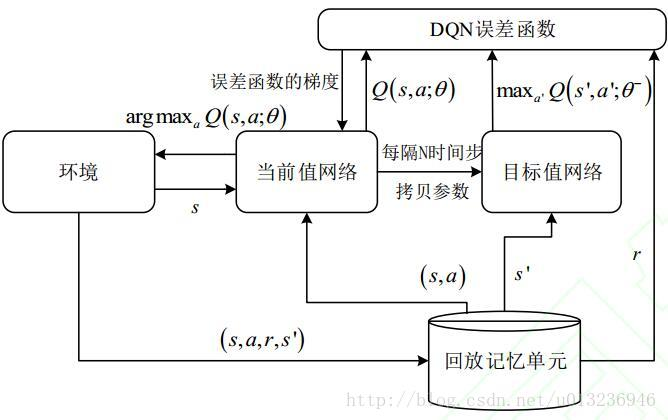
\includegraphics[width=0.9\textwidth]{liuchengtu_DQN}
\caption{DQN流程图}
\label{fig:liuchengtu_DQN}
\end{figure}

从图中,我们可以看出,DQN的主要学习过程包括以下几步:

(1)构建回放记忆单元。在每个情节中,初始化第一个状态$s$,并在接下里的每个时间点,按照$\epsilon-greedy$选择行为$a$,然后在仿真器中执行,可以得到即时奖赏$r$,下一步的状态$s^{'}$。并将此转换样本($s,a,r,s^{'}$)放到回放构建单元中。

(2)值函数的学习。从回报记忆单元中随机选取一条转移记录($s,a,r,s^{'}$),并分别使用当前值网络和目标值网络分别计算出值函数的估计值 $Q(s,a;\mathbf{\theta})$和TD目标值$r+\gamma \max_{s^{'}}Q(s^{'},a^{'};\mathbf{\theta^{-}})$,然后求出损失函数$L=(r+\gamma \max_{s^{'}}Q(s^{'},a^{'};\mathbf{\theta^{-}})-Q(s,a;\mathbf{\theta}))^{2}$,并使用梯度下降法进行求解。具体的损失函数参见图$\ref{fig:liuchengtu_DQN}$

(3)更新目标网络参数。经过若干步的训练后,将估计网络的参数拷贝给目标网络参数。

\begin{figure}[htbp]
\centering
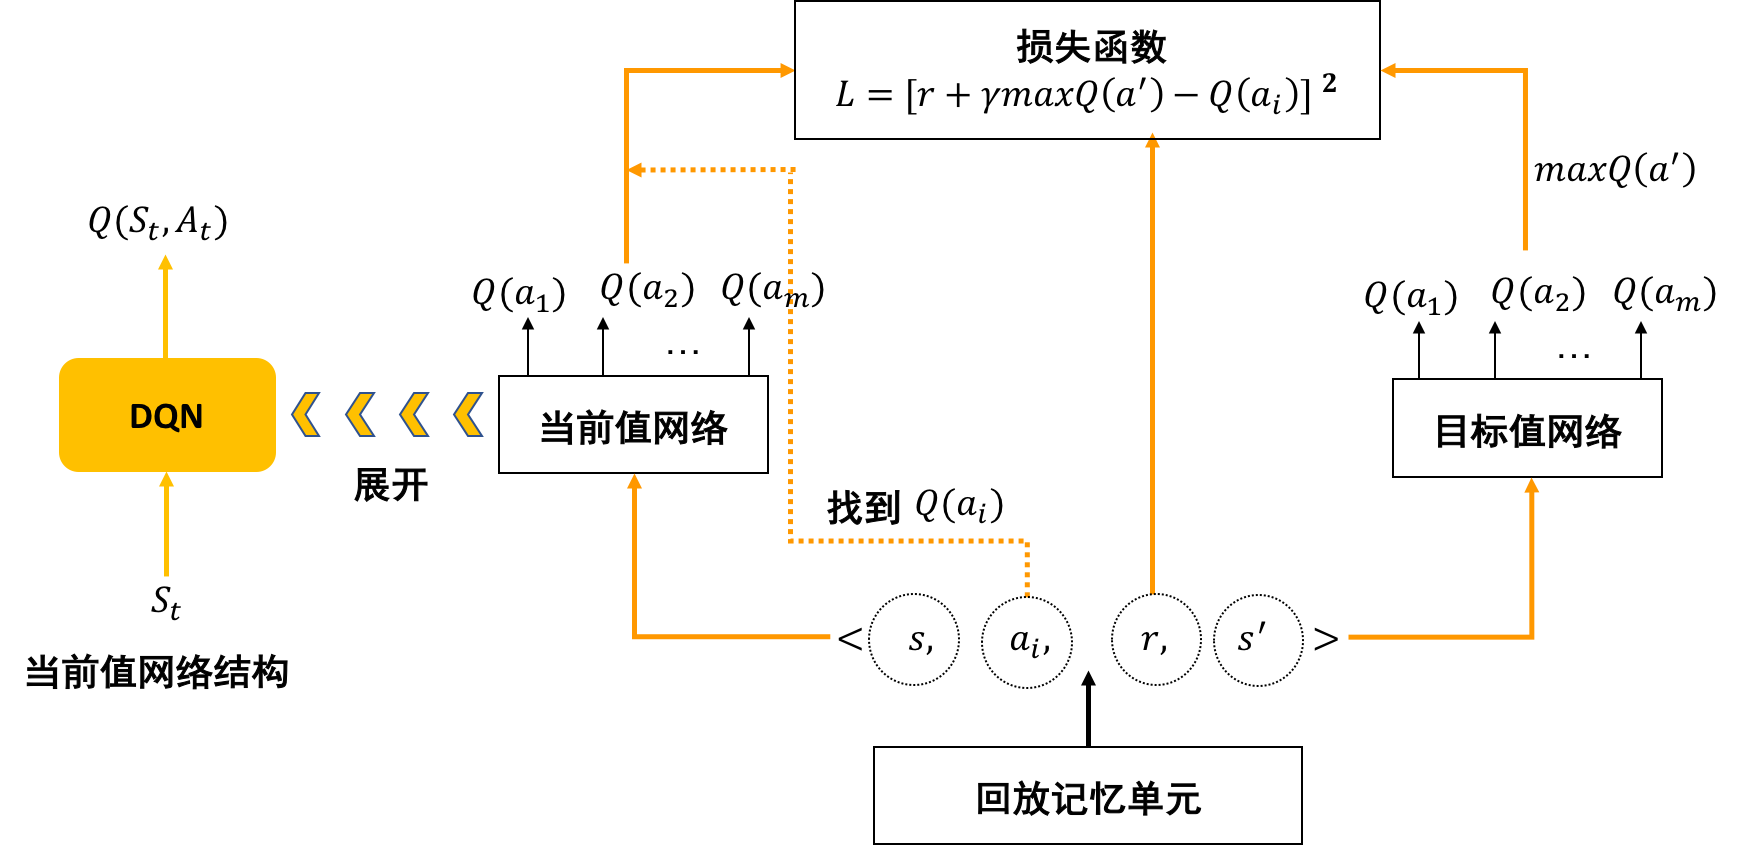
\includegraphics[width=0.8\textwidth]{loss_DQN}
\caption{DQN损失函数构造}
\label{fig:loss_DQN}
\end{figure}

结合算法$\ref{algo:algorithm_2}$,我们可以得出DQN算法的具体过程,其伪代码如算法$\ref{algo:algorithm_DQN}$所示。
\begin{algorithm}[htbp]
\small
\SetAlgoLined
\SetKwRepeat{Repeat}{repeat}{until} 
初始化回放记忆库$D$,记忆库大小为$N$\;
利用随机权值$\mathbf{\theta}$初始化状态行为值函数$Q$\;
初始化$\mathbf{\theta}^{-}$令$\mathbf{\theta}^{-}=\mathbf{\theta}$,用以计算TD目标的状态行为值$\hat{Q}$\;
\For{$episode=1,\cdots, M$}{
	初始化情节的第一个状态:$s_{1}={x_{1}}$(${x_{1}}$为环境的观测特征),通过预处理得到状态对应的特征输入:$\phi_{1}=\phi(s_{1})$\;
	\For{$t=1,\cdots, T$}{
		以概率$\epsilon$选一个随机行为$a_{t}$\;
		如果以上小概率事件没有发生,则按照贪婪策略选择当前值函数最大的那个行为:$a_{t}=\argmax_{a}Q(\phi(s_{t}),a;\mathbf{\theta})$\;
		在仿真器中执行行为$a_{t}$,可以观测到奖赏$r_{t}$以及下一步的环境的观测特征\;
		设置$s_{t+1}=s_{t},a_{t},x_{t+1}$,预处理得到对应的特征输入:$\phi_{t+1}=\phi(s_{t+1})$\;
		将转换样本($\phi_{t}, a_{t}, r_{t}, \phi(s_{t+1})$)放到回放记忆库中\;
		从回放记忆库D中均匀随机采样一个转换样本数据($\phi_{j}, a_{j}, r_{j}, \phi(s_{j+1})$)\;
		判断是否是一个情节的终止状态,若是,则TD目标位$r_{j}$,否则利用TD目标网络$\mathbf{\theta}^{-}$计算TD目标$r+\gamma \max_{s^{'}}Q(s^{'},a^{'};\mathbf{\theta^{-}})$\;
		执行一次梯度下降算法:$\triangle \theta = \alpha [r+\lambda \max_{a^{'}}Q(s^{'},a^{'};\theta^{-})-Q(s,a;\theta) ]\triangledown_{Q}(s,a;\mathbf{\theta})$\;
		更新状态行为值函数逼近的网络参数:$\mathbf{\theta}=\mathbf{\theta}+\triangle \theta$\;
		每隔$C$步更新一次TD目标网络权值;即:$\mathbf{\theta}^{-}=\mathbf{\theta}$\;
	}
}
% 输出最终策略:$\pi(s)=\argmax_{a}Q(s,a)$\;
\caption{DQN伪代码}
\label{algo:algorithm_DQN}
\end{algorithm}


\section{基于LSTM的深度强化学习混合模型设计}
\subsection{RNN和LSTM}
在DQN中,值函数逼近所使用的是卷积神经网络,它的结构有一个特点:就是假设输入是一个独立的没有上下文联系的单位。但是在序列化问题中,前面的输入和后面的输入是有关系的,也就是要具有针对长时间信息的记忆功能。所以,我们考虑使用循环神经网络(recurrent neural networks,RNN)和它的改进版本长短时记忆网络(ong short-term memory,lstm)来学习强化学习中状态的表示。因为循环网络的模型可以聚合过去的部分信息,并且可以捕捉到序列的长短时依赖性。因此,在处理序列问题上,它们的表现要优于卷及神经网络的性能。
 \paragraph{RNN}
RNN(Recurrent Neuron Network)是一种对序列数据建模的神经网络,即一个序列当前的输出与前面的输出也有关。具体的表现形式为网络会对前面的信息进行记忆并应用于当前输出的计算中,即隐藏层之间的节点不再无连接而是有连接的,并且隐藏层的输入不仅包括输入层的输出还包括上一时刻隐藏层的输出。图$\ref{fig:rnn}$是一个RNN模型的示例图。
\begin{figure}[htbp]
\centering
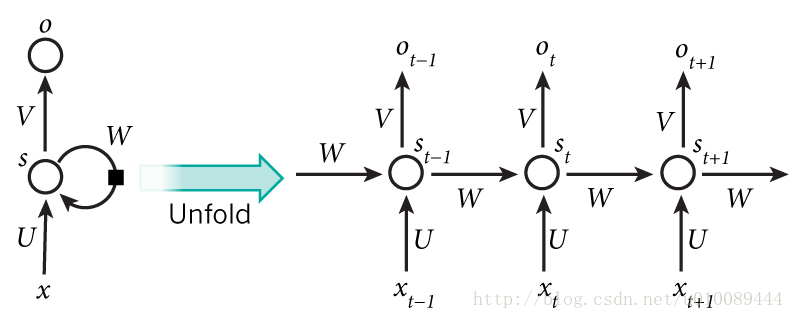
\includegraphics[width=0.8\textwidth]{rnn}
\caption{rnn模型}
\label{fig:rnn}
\end{figure}

在图$\ref{fig:rnn}$中:$x_{t}$表示$t$时刻的输入。$s_{t}$是$t$时刻的隐状态(memory),基于上一时刻的隐状态和当前输入得到:$s_t=f(U x_{t}+W s_{t−1})$,其中$f$一般是非线性的激活函数,在计算$s_{0}$时,即第一个单词的隐藏层状态,需要用到$s_{−1}$,但是其并不存在,在实现中一般置为0。$o_{t}$表示$t$时刻的输出。$\mathbf{U}$是输入层到隐藏层的权重矩阵,$\mathbf{V}$是隐藏层到输出层的权重矩阵,权重矩阵$\mathbf{W}$就是隐藏层上一次的值作为这一次的输入的权重。需要注意的是:在传统神经网络中,每一个网络层的参数是不共享的。而在RNN中,所有层次均共享同样的参数(例如上例中的$\mathbf{U}$,$\mathbf{V}$,$\mathbf{W}$)。其反应出RNN中的每一步都在做相同的事,只是输入不同,因此大大地降低了网络中需要学习的参数。

这个网络在$t$时刻接收到输入$x_{t}$之后,隐藏层的值是$s_{t}$,输出值是$o_{t}$。特别的,$o_{t}$的值不仅仅取决于$x_{t}$,还取决于$o_{t-1}$。我们可以用下面的公式来表示循环神经网络的计算方法:
\begin{equation}
\label{rnn_1}
\begin{aligned}
o_{t}=g(\mathbf{V}s_{t})
\end{aligned}
\end{equation}
\begin{equation}
\label{rnn_2}
\begin{aligned}
s_{t}=f(\mathbf{U}x_{t}+\mathbf{W}s_{t-1})
\end{aligned}
\end{equation}
式\eqref{rnn_1}是输出层的计算公式,输出层是一个全连接层,也就是它的每个节点都和隐藏层的每个节点相连。$\mathbf{V}$是输出层的权重矩阵,$g$是激活函数。式\eqref{rnn_2}是隐藏层的计算公式,它是循环层。$\mathbf{U}$是输入$x$的权重矩阵,$\mathbf{W}$是上一次的值作为这一次的输入的权重矩阵,$f$是激活函数。

从上面的公式我们可以看出,循环层和全连接层的区别就是循环层多了一个权重矩阵$\mathbf{W}$。

如果反复把式$\eqref{rnn_2}$带入到式$\eqref{rnn_1}$,我们将得到:
\begin{equation}
\begin{aligned}
o_{t}&=g(\mathbf{V}s_{t})\\
&=\mathbf{V}f(\mathbf{U} x_{t}+\mathbf{W} s_{t-1})\\
&=\mathbf{V}f(\mathbf{U} x_{t}+\mathbf{W} f(\mathbf{U} x_{t-1}+\mathbf{W} s_{t-2}))\\
&=\mathbf{V}f(\mathbf{U} x_{t}+\mathbf{W} f(\mathbf{U} x_{t-1}+\mathbf{W} f(\mathbf{U} x_{t-2}+\mathbf{W} f(\mathbf{U} x_{t-3}+\cdots)))\\
\end{aligned}
\end{equation}

从上面可以看出,循环神经网络的输出值$o_{t}$,是受前面历次输入值$x_{t}$、$x_{t-1}$、$x_{t-2}$、$x_{t-3}$、$\cdots$影响的,这就是为什么循环神经网络可以往前看任意多个输入值的原因。

循环神经网络的训练方法可以采用基于时间的反向传播算法(Backpropagation through time, BPTT),具体的更新方法和BP更新方法相同。但是,在处理较长序列的时候,普通循环神经网络不能得到较好的性能。一个主要原因是,RNN在训练中如果向前考虑的很远的时候,会导致对应的误差项的值增长或者缩小的非常快,就会很容易发生梯度爆照或者梯度消失的现象,这导致训练时梯度不能在较长序列中一直传递下去,从而使RNN无法捕捉到长距离的影响。

通常来说,梯度爆炸更容易处理一些。因为梯度爆炸的时候,我们的程序会收到NaN错误。我们也可以设置一个梯度阈值,当梯度超过这个阈值的时候可以直接截取。梯度消失更难检测,而且也更难处理一些,除了合理的初始化权重值、使用relu代替sigmoid和tanh作为激活函数外,还可以使用其他诸如长短时记忆网络(LTSM)的方法。其中后者是目前最流行的方法。

 \paragraph{LSTM}
原始RNN的隐藏层只有一个状态,它对于短期的输入非常敏感,LSTM在此基础上增加了一个状态,让它保存长期的状态。从而解决了传统RNN无法处理长距离依赖的问题。新增加的状态称为单元状态(cell state)。

如图$\ref{fig:lstm_2}$所示为lstm的展开结构,灰色矩形部分是一个lstm的简化结构,其中h为原始RNN的隐藏层状态,c为单元状态。从图中我们可以看出,在t时刻,LSTM的输入有三个:当前时刻网络的输入值$x_{t}$、上一时刻LSTM的输出值$h_{t-1}$、以及上一时刻的单元状态$c_{t-1}$;LSTM的输出有两个:当前时刻LSTM输出值$h_{t}$、和当前时刻的单元状态$c_{t}$。注意$x$、$h$、$c$都是向量。LSTM的关键就是怎样控制长期状态c。在这里,LSTM的思路是使用三个控制开关。第一个开关,负责控制继续保存长期状态c;第二个开关,负责控制把即时状态输入到长期状态c;第三个开关,负责控制是否把长期状态c作为当前的LSTM的输出。
\begin{figure}[htbp]
\centering
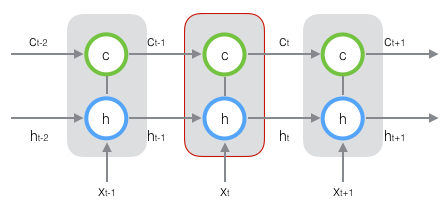
\includegraphics[width=0.8\textwidth]{lstm_2}
\caption{LSTM按时间维度展开图}
\label{fig:lstm_2}
\end{figure}
如图$\ref{fig:lstm}$为LSTM神经内部结构。上述表述的开关在LSTM中使用的门(gate)来实现的,门实际上就是一层全连接层,它的输入是一个向量,输出是一个0到1之间的实数向量。假设$W$是门的权重向量,$b$是偏置项,那么门可以表示为:
\begin{displaymath}
\begin{aligned}
g(x)=\sigma (W x+b)
\end{aligned}
\end{displaymath}
门的使用,就是用门的输出向量按元素乘以我们需要控制的那个向量。因为门的输出是0到1之间的实数向量,那么,当门输出为0时,任何向量与之相乘都会得到0向量,这就相当于啥都不能通过;输出为1时,任何向量与之相乘都不会有任何改变,这就相当于啥都可以通过。因为$\sigma$(也就是sigmoid函数)的值域是(0,1),所以门的状态都是半开半闭的。

LSTM用两个门来控制单元状态c的内容,一个是遗忘门(forget gate),它决定了上一时刻的单元状态$c_{t-1}$有多少保留到当前时刻;另一个是输入门(input gate),它决定了当前时刻网络的输入$x_{t}$有多少保存到单元状态。LSTM用输出门(output gate)来控制单元状态$c_{t}$有多少输出到LSTM的当前输出值$h_{t}$。

遗忘门:
\begin{equation}
\begin{aligned}
f_{t}=\sigma (\mathbf{W}_{f} \cdot [h_{t-1}, x_{t}]+b_{f})
\end{aligned}
\end{equation}

上式中,$\mathbf{W}_{f}$ 是遗忘门的权重矩阵,$[h_{t-1}, x_{t}]$表示把两个向量连接成一个更长的向量,$b_{f}$是遗忘门的偏置项,$\sigma$是sigmoid函数。

输入门:
\begin{equation}
\begin{aligned}
i_{t}=\sigma (\mathbf{W}_{i} \cdot [h_{t-1}, x_{t}]+b_{i})
\end{aligned}
\end{equation}
上式中,$\mathbf{W}_{i}$是输入门的权重矩阵,$b_{i}$是输入门的偏置项。

用于描述当前输入的单元状态$\tilde{c}_{t}$,它是根据上一次的输出和本次输入来计算的:
\begin{equation}
\begin{aligned}
\tilde{c}_{t}=\tanh (\mathbf{W}_{c} \cdot [h_{t-1}, x_{t}]+b_{c})
\end{aligned}
\end{equation}

计算当前时刻的单元状态$c_{t}$:
\begin{equation}
\begin{aligned}
c_{t}=f_{t} \circ c_{t-1} + i_{t} \circ \tilde{c}_{t}
\end{aligned}
\end{equation}
上式中,符号$\circ$表示按元素乘。它是由上一次的单元状态$c_{t-1}$按元素乘以遗忘门$f_{t}$,再用当前输入的单元状态$\tilde{c}_{t}$按元素乘以输入门$i_{t}$,再将两个积加和产生的。我们就把LSTM关于当前的记忆$\tilde{c}_{t}$和长期的记忆$c_{t-1}$组合在一起,形成了新的单元状态$c_{t}$。由于遗忘门的控制,它可以保存很久很久之前的信息,由于输入门的控制,它又可以避免当前无关紧要的内容进入记忆。

输出门,它控制了长期记忆对当前输出的影响:
\begin{equation}
\begin{aligned}
o_{t}=\sigma(W_{\sigma} \cdot [h_{t-1}, x_{t}]+b_{o})
\end{aligned}
\end{equation}

LSTM最中的输出,是由输出门和单元状态共同确定的:
\begin{equation}
\begin{aligned}
h_{t}=o_{t} \circ \tanh(c_{t})
\end{aligned}
\end{equation}

以上就是LSTM的前向计算。
\begin{figure}[htbp]
\centering
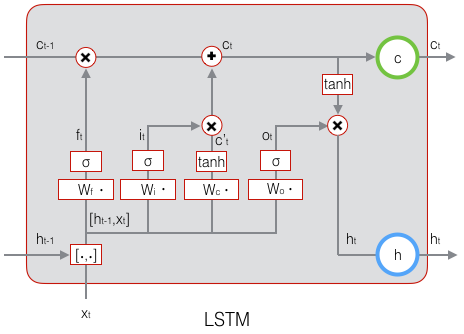
\includegraphics[width=0.8\textwidth]{lstm}
\caption{LSTM内部结构}
\label{fig:lstm}
\end{figure}

关于LSTM的训练过程仍然采用的反向传播算法,因为篇幅的限制具体计算过程不详细展开,主要包括以下三步:

(1)前向计算每个神经元的输出值,对于LSTM来说,即 $\mathbf{f}_{t}$、$\mathbf{i}_{t}$、$\mathbf{c}_{t}$、$\mathbf{o}_{t}$、$\mathbf{h}_{t}$五个向量的值。。

(2)反向计算每个神经元的误差项值。与循环神经网络一样,LSTM误差项的反向传播也是包括两个方向:一个是沿时间的反向传播,即从当前t时刻开始,计算每个时刻的误差项;一个是将误差项向上一层传播。

(3)根据相应的误差项,计算每个权重的梯度。


\subsection{一步混合模型}
% 就像第一节所描述的那样,因为强化学习考虑到了未来的回报,而且它的目标是直接优化长期奖赏,这与在直复营销场景中所期望的最大化客户ltv的目标是一致的。
基于RNN的深度强化学习模型(RL-RNN和RL-LSTM)在模型的的计算和训练上与DQN是类似的,但是因为循环神经网络通过对未来奖赏的长短时依赖性进行建模从而可以更好的处理序列中的部分可观测问题的原因,被广泛应用在序列问题的处理上\citep{bakker2002reinforcement,hausknecht2015deep,lin1993reinforcement,narasimhan2015language}。它们所设计的模型可以使用图$\ref{fig:rl_rnn}$表示。

在图$\ref{fig:rl_rnn}$中,$o_{t}$是观测值,$\tilde{h}_{t}$为RNN的隐藏状态,此处的当前隐藏状态是对其内部历史信息的概要总结。$Q(s,a)_{t}$是在时间$t$下采取行为$a$并且状态$s$为$\tilde{h}_{t}$的预测Q值。即Q网络是关于当前观测$o_{t}$和当前内部历史概要信息(隐藏层)$\tilde{h}_{t-1}$的函数,随着时间的推移,内部历史信息$\tilde{h}_{t}$将循环的更新,当Q网络学习完毕后,以贪婪的方式选择最优的行为。
\begin{figure}[htbp]
\centering
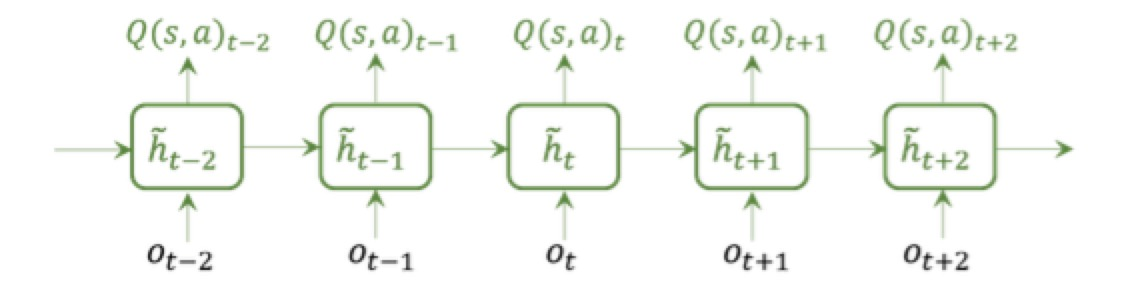
\includegraphics[width=1.0\textwidth]{rl_rnn}
\caption{RL-RNN框架}
\label{fig:rl_rnn}
\end{figure}

在RL-RNN模型中,因为RNN网络具有捕捉长期依赖性的强大能力,所以可以较好的估计Q函数。但是,在网络优化的过程中,RNN还需要可以很好的解决部分可观测的问题,那么如果要同时达到这两个目的,对于只有一个网络结构的RL-RNN来说是很难的。

所以,我们可以考虑具有两个网络的混合模型。可以使用强化学习模型,最大限度的获得长期回报,同时,可以对观测值和即刻奖赏的预测以训练优化监督学习模型,从而具有更好的推断和表示隐藏状态的能力。在这种混合方法中,使用监督学习来进行隐藏状态的表示学习,使用强化学习进行策略的学习,通过强化学习和监督学习的优势互补,可以使的这种混合模型达到很好的预测效果。另外,需要特别强调的是,这两个模型不能单独进行优化,而应该在监督学习了一个内部隐状态表示后就用强化学习模型最大化长期的奖赏。

使用以上混合模型的思想,我们可以得到基于rnn(lstm)和dqn的混合模型,即用rnn(lstm)进行监督模型的训练,使用dqn进行强化学习的训练,我可以将模型记为SL-RNN-RL-DQN(SL-LSTM-RL-DQN)。混合模型的网络结构如图$\ref{fig:rnn_dqn}$所示:
\begin{figure}[htbp]
\centering
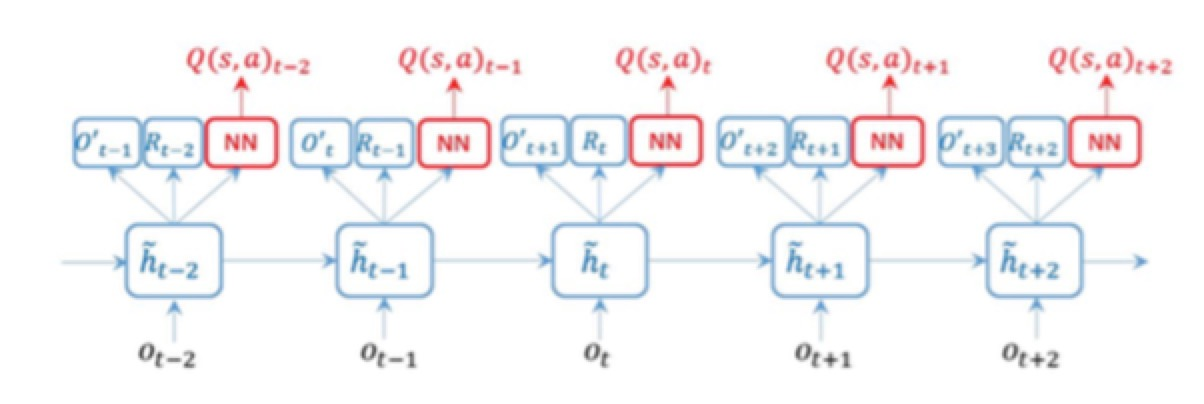
\includegraphics[width=1.0\textwidth]{rnn_dqn}
\caption{rnn-dqn框架}
\label{fig:rnn_dqn}
\end{figure}

在图$\ref{fig:rnn_dqn}$中,$o_{t}$是观测值,$h_{t}$是RNN的隐藏状态,$o_{t+1}^{'}$是$t+1$ 时刻的预测的观测值,$R_{t}$是预测的奖赏。$Q(s,a)_{t}$是t时刻预测的Q值,蓝色部分对应着RNN的监督学习部分,红色部分对应着DQN的学习部分。在混合模型中,DQN的输入是有监督的RNN模型。在训练阶段,我们使用联合训练的方法,首先我们在一个时刻从下一步的观测值和即时奖赏的信号中训练rnn(或者lstm)以学习隐藏状态的表示方法,然后,将学习到的隐藏状态作为DQN的输入,去学习近似最优策略的Q函数。以上这两个训练步骤在随机梯度下降迭代过程中交错进行。

因为在RNN-DQN学习的全部过程中,监督学习和强化学习模型按照上述训练方法依次进行学习,在学习过程中没有发生网络结构的变化,因此我们称之为一步混合模型,记为1-RNN-DQN。

由此,我们可以得到1-RNN-DQN模型的流程图以及损失函数的构造图。

\subsection{两步混合模型}
在上述的1-RNN-DQN模型中,先使用监督模型rnn进行隐藏状态的表示学习,再使用dqn进行策略的学习。在训练的过程中,监督信号将学习到的状态信息,反向传播到rnn或者lstm的头部,而强化学习只是将误差信号反向传播到rnn隐藏层,不参加rnn的训练。这种独立的训练方法虽然可以加快网络的训练速度,但是,因为两部分的误差信号是没有联系的,所以会造成这两部分网络的训练不平衡,从而影响最终的预测性能。这种不平衡性主要表现在1)rnn网络训练的不充分性影响了dqn的训练结果,从而造成了在rnn网络没有得到很好的隐状态表示时,但是dqn网络可能已经基于这种不好的表示而完成了较好的训练。2)即使两部分的网络都已经很好的完成了训练,但是这种割裂的误差传播仍然影响最终的表现。

基于以上的想法,我们提出了两步混合模型,记为2-RNN-DQN。在2-RNN-DQN中分为两个阶段,第一阶段按照2-RNN-DQN的方法进行训练,学习到两个网络的参数向量$\mathbf{\omega_{'}}$和$\mathbf{\omega_{''}}$,第二阶段将rnn网络的隐藏层和dqn网络的输入层连接起来,组成一个新的网络$[\mathbf{\omega_{'}},\mathbf{\omega_{''}}]$。新的网络的输入是观测值,输出是Q函数。具体学习过程是:将观测值输入到新的网络中,输出一个估计得Q值,然后利用误差学习更新整个网络的参数。

算法流程图如下。

\subsection{对照实验模型}

到目前为止,我们已经得到了DQN、RL-RNN、RL-lstm、1-SL-RNN+RL-dqn、1-SL-lstm+RL-dqn、2-SL-RNN+RL-dqn、2-SL-lstm+RL-dqn的模型的方法,作为对照组,我们提供了监督学习的训练方法。

在监督学习的模型中,我们的目标是从给定的到目前为止的交互历史中,预测可以导致更高的即刻奖赏的行为。在我们的实验中,我们使用原始奖赏信号作为目标进行回归预测。对于训练数据中的任意一个转移样本($o,a,r,o_{'}$),我们需要学习在给定观测o下奖赏r的回归曲线。我们主要考虑一下三个模型。

多层深度神经网络模型。该模型将交互历史分成单个的转移样本${(o_{t}, a_{t}, r_{t}, o_{t+1})}_{t=1,2,\cdots}$,基于($o_{t},a_{t}$)来学习预测$r_{t}$。这个模型使用$\hat{R}$来表示,在测试过程中,将目前的观测量$o$作为输入,通过奖赏的预测贪婪的选择行为:$\argmax_{a}\hat{R}(s,a)$。

RNN和LSTM可以从历史的交互中对长期依赖性进行建模。像图$\ref{fig:rnn_}$所示,$o_{t}$为观测值,$\tilde{h}_{t}$为rnn的内部状态,$R(s,a)_{t}$为在$t$时刻的预测的奖赏值,其中$s$是rnn的$\tilde{h}_{t}$。客户的交互历史不再像DNN那样被分解为单一的转移样本。在t时刻,这个模型使用观测值$o_{t}$,奖赏$r_{t}$以及目前的内部历史总结$\tilde{h}_{t-1}$来进行更新,并且在rnn中循环的保持这种更新方式。在测试阶段,模型基于当前的观测值和当前的内部历史概要信息来选择行为。lstm的过程和rnn过程类似。
\begin{figure}[htbp]
\centering
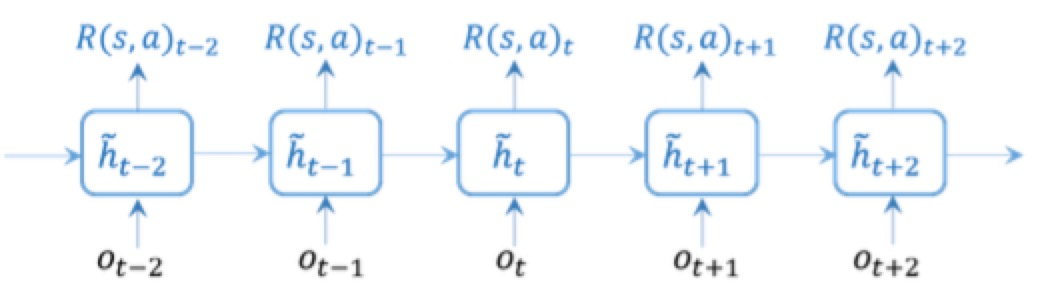
\includegraphics[width=1.0\textwidth]{rnn_}
\caption{rnn训练展开图}
\label{fig:rnn_}
\end{figure}

\section{本章小结}


\chapter{SVR+Q+MCKP分块逼近模型在广告预算分配中的研究}

% 首先介绍多渠道广告投放资金分配问题使用强化学习研究的现状(没有利用强化学习解决该问题的文献,存在的主要问题:数据量较少,导致值函数估计不准确等问题,收敛速度慢,说明本文采用非参数化建模的原因,非参数化建模又存在什么问题,针对此问题又是如何解决的)
% 介绍深度强化学习
% 介绍本文提出的混合网络模型算法
% “我知道我的广告费有一半浪费了,可是我不知道浪费的是哪一半。”美国费城商人约翰·华纳梅克的这句自嘲式的调侃简直让人抓狂——似乎你绞尽脑汁想出的营销点子就是为了达到一个目的——尽量让广告费被浪费得少一点而已。

\section{直复营销下广告预算分配问题阐述}
这一节,首先介绍了在直复营销体系下,基于第三方广告代理商进行广告投放的应用场景及其具体的投放过程。然后,说明了多渠道广告投放的目标是追求全渠道的LTV最大化,以此作为选择强化学习解决该问题的依据。最后,介绍了在广告投放预算分配场景中所面临的三个特点,并针对这些特点进行分析,提出对应的解决思路,来作为本章研究的出发点。

\subsection{广告预算分配场景}
美国直复营销协会(American Direct Marketing Association,ADMA)\footnote{http://www.the-dma.org/}将直复营销(Direct Response Marketing)定义为一种市场营销体系,运用一种或几种广告媒介在任何地点产生可以度量的反应或交易。直效营销仅仅属于直复营销中的一种应用场景,它特指不通过第三方,中间人,而直接对客户进行推广和营销,以维持企业与客户的良好关系。但是,在此场景下需要企业有充足的客户资源和大量的相关客户资料,这对于大部分企业是很难办到的,因为它需要很长时间的积累,特别是在日益激烈的市场竞争环境中,时间就是企业的生命。于是,为了快速获取用户、推广相关产品、扩大公司的收入,越来越多的企业选择通过第三方广告代理商(ad-agency)进行广告投放。

广告代理商除了帮助企业进行广告设计与策划以外,还有一部分更重要的工作,就是帮助广告主安排或代为购买媒介空间或时间。近年来,随着广告市场的不断发展和扩大,为了方便广告主高效的进行广告投放,大部分在线的广告代理商都建设了自己的广告投放平台,其投放流程如图
% $\ref{fig:ad_process}$
所示:在广告投放平台上,广告代理商(ad-agency)有很多可供选择的广告渠道(channel)资源,广告主在每次进行广告投放时需要提供一个广告投放策略,策略的内容包括在哪些渠道上投放广告以及对应投放多少金额的广告费。然后,广告代理商会按照广告主提供的投放策略,将相应的广告投放量通过各渠道投放给潜在顾客(广告的受众)。在广告投放结束后,广告代理商会将此次广告投放的直观效果反馈给广告主,同时广告主也可以通过追踪已经产生交易的顾客的后续信息,综合评价此次的投放效果。



通过以上的介绍,可以看到,在通过广告代理商投放广告的过程中,顾客可以及时接收到广告主发布的广告信息,而广告主也会收到响应顾客的响应反馈,因此广告主与顾客之间是存在互动性的。另外,广告主还可以根据广告代理商反馈的投放效果信息以及追踪用户未来的交易等方式去量化此次广告投放对企业的价值,因此效果是可衡量性的,所以,利用广告代理商进行广告投放的方式也属于直复营销体系的研究范围内。

在企业进行广告投放的真实业务中,为了保证财务帐面的稳定以及公司合理健康的发展,公司财务每个月都会提前给出该月的广告投放资金的预算,然后广告投放部门会在此预算下进行广告预算的合理分配,以使得公司的业务不断扩大、收入持续增长。但是,因为广告投放场景比较复杂,单纯靠广告投放人员制定预算分配策略往往很持续难达到好的效果,所以需要充分利用机器学习技术协助进行决策。

\subsection{基于全渠道的LTV值}
通常情况下,企业在进行广告投放时,为了能够更好的评价广告渠道的质量,而且为了能达到持久有效的营销效果,一般都会选择一个广告代理商进行为期一年或几年的持续投放。因此,广告投放是一个序列化的过程。

评价广告投放渠道质量的重要指标是该渠道的投资回报比(Return On Investment, ROI),即一定周期内,广告主通过广告投
放收回的价值占广告投入的百分比,计算方法如式\eqref{seq:roi}所示,其中Income表示收入额,Cost表示成本额,Investment表示投资额,一般情况下认为Cost和Investment是同一概念。
\begin{equation}\label{seq:roi}
\begin{aligned}
 ROI=\frac{Income-Cost}{Investment} \times 100\%
\end{aligned}
\end{equation}

然而,在广告投放的过程中,用户的反馈存在一定的延迟,而且某一时刻投放的广告会对后面时刻的广告投放效果产生一定程度的影响,所以不能仅仅使用即时的ROI值作为渠道质量的评价指标。比如,一个顾客在某一时刻看到某广告,但是并没有立刻产生正向反馈或者交易,而是在经过若干时间后的某一时刻才有正向反馈。那么,此时所产生的收益不单单与现在这个时刻的广告投放效果有关,还与之前的广告投放效果有关。所以,在计算广告投放所产生的回报时,应该要有全局观念。因此,在实际应用中,广告主一般将基于渠道LTV的ROI值作为选择广告渠道的指标,LTV是指渠道所产生的累积收益,只要将公式\eqref{seq:roi}中的Income换成渠道的LTV值即可。

考虑到企业进行广告投放的主要目的是为了尽可能的增加自身利润,如果单单只考虑渠道的ROI值,并不能得到对企业来说价值最大的投放策略。因为即使一个投放产生的ROI值很大,但是如果产生这个很大ROI值的那个投放花费很小的话,其利润不可能很大,这并不是企业所期望得到的最终效果。所以本章研究的给定预算下的广告投放资金分配问题,并不以ROI值作为评价指标,而是关注什么样的投放策略可以使企业产生的收益最大化,即广告渠道的LTV值最大化。

通过第二章的介绍,我们知道,强化学习在处理序列问题时,因为考虑到了延迟奖赏的问题,并且以追求累积奖赏最大化作为优化目标,所以将强化学习技术应用在广告投放领域,可以充分发挥其优势。

\subsection{广告预算分配特点}
% 多渠道/总预算限制/数据量少
解决好广告投放的资金预算分配问题,虽然有着很高的现实意义和商业价值,但是目前并没有引起很多学者和专家的注意。其中,最主要的原因就是没有在此领域公开的数据集。本文的数据是基于国内某公司在进行广告投放过程中所产生的真实数据,所以研究内容具有的实用性和真实性。

即便拥有了相关的广告投放数据,但是因为该领域还存在诸如场景复杂、数据量较少、固定预算约束等问题,不能直接将强化学习算法应用在该场景中。所以,本章从这些存在的问题作为出发点,结合强化学习进行分析,并提出了相应的解决方法。

对于大部分企业来说,广告投放是以天为单位进行的,所以投放数据量比较少,影响了模型的训练和学习,因此,为了提高数据的使用率,在强化学习模型中我们考虑使用非参数化函数逼近的方法进行Q值函数的学习。另外,通常情况下,为了达到全方位的效果,在进行广告投放时会选择多个渠道同时进行投放,因此,我们不能只考虑渠道自身的延迟反馈影响,而且还应该考虑渠道间的相互影响。最后,每一次的广告投放策略都需要在给定的固定预算约束进行,所以,我们在使用强化学习进行Q值估计之后,还要考虑如何进行合理的分配方法。

\section{SVR+Q+MCKP模型}
为了解决多渠道广告预算的资金分配问题,在我们的模型中,首先需要使用强化学习算法估算出当前时刻每一个渠道在每一种花费下可能产生的累积利润(即Q值),然后,再利用多选择背包问题(Multiple-Choice Knapsack Problem, MCKP)选择出每个渠道最合适的花费以使的企业产生的利润最大化。

然而,在真实的广告投放场景中,广告主进行广告投放的周期是相对较长的(一天一次),所能得到的数据也就相对较少。所以,在进行Q值函数逼近值时,要求我们高效的利用仅有的训练样本。然而,通过第二章的介绍,我们知道在参数化函数逼近方法中,线性逼近值函数的逼近能力较弱、效率较低,非线性函数(神经网络)逼近又需要有充足的训练样本。所以,综合考虑,我们选择了基于非参数化函数逼近的模型,因为该模型是一种基于样本的学习方法,具有较高的灵活性,而且适用于小样本数据。

但是,非参数化函数逼近常常存在着收敛性难移保证的问题。于是,本章提出了基于SVR+Q的分块强化学习模型,在该模型中,将对Q值函数逼近问题转化为高维特征空间中的线性回归问题,从而可以加快函数的收敛速度。另外,为了在小数据集下提高函数逼近的精度,提出分块逼近的思想,每个离散的行为作为一块,分别使用SVR+Q模型进行训练,最后再利用训练好的分块模型多路逼近Q值函数。在训练结束后,再使用MCKP问题解决资金的合理分配问题。

\subsection{问题的形式化定义}
下面给出多渠道广告投放预算分配问题的形式化描述:

假定在多渠道广告投放中给定的固定预算金额为$B$,广告投放的策略$\bm{x}=(x_{1},x_{2},\cdots,x_{n})$,即$x_{i}$是在第$i$个渠道上分配的投放金额,$n$为渠道的数量。令$R(\bm{x})$是在给定预算分配策略$\bm{x}$下的累积利润。所以,我们可以将问题形式化描述为:
\begin{equation}\label{seq_ad_goal}
\begin{split}
&max_{\bm{x}} R(\bm{x}),\\
&s.t. \sum_{i=1}^{n} x_{i} \leqslant B \text{且} x_{i} \geq 0.
\end{split}
\end{equation}

也就是说,我们的目标是将预算金额$B$在$n$个渠道上进行合理划分,以使得整体收益最大化。但是,在进行划分前,我们需要清楚的知道当前时刻每一个渠道在每一种可能的花费下会产生什么样的价值(累积利润)。这里,我们采用的是基于SVR+Q多路分块逼近强化学习模型。

\subsection{分块多路逼近思想}
经过前面的分析,我们知道,在广告投放场景中,可获得的数据量比较少,如果将所有渠道合在一起进行建模,很难拟合出可靠的值函数变化规律。所以,我们采取分渠道进行建模的思路。进一步地,每个渠道在进行值函数的逼近时,考虑到状态空间和行为空间(广告花费)是连续的,因为数据样本较少也会造成状态行为值函数逼近的不准确。

针对上述第二个问题,本章提出分块多路逼近的思想。在离线学习时,首先,使用一种花费空间离散化的方法(第三节会详细介绍该方法),将花费空间离散成$K$个行为$A=\{a_{1},a_{2},\cdots,a_{K}\}$。然后,将花费$c_{t}$所对应的离散行为$a_{t}$加入到原始训练样本<$\mathbf{s}_{t},c_{t},r_{t+1},\mathbf{s}_{t+1}$>中,并且按照样本中行为的类别将原始样本集划分为$K$个临时样本单元(即$K$个块),所以,每一个离散行为$a_{k}$对应一个临时样本单元$D_{k}^{'}=\{<\mathbf{s}_{t},c_{t},a_{t},r_{t+1},\mathbf{s}_{t+1}>|t=1,2,\cdots,N_{k}\}$,$N_{k}$为该临时样本单元$D_{k}^{'}$中的样本个数,$\mathbf{s}_{t}$为当前状态向量,$\mathbf{s}_{t+1}$为后继状态向量。接着,针对每一个临时样本单元$D_{k}^{'}$,利用Q值函数的更新公式(算法$\ref{algo:algorithm_2}$中第7行)计算$Q(\mathbf{s_{t}})$值,形成带Q值的样本单元$D_{k}=\{<\mathbf{s}_{t},a_{t},r_{t+1},Q(\mathbf{s}_{t}),\mathbf{s}_{t+1}>|t=1,2,\cdots,N_{k}\}$。下一步,利用非参数化函数逼近模型Q对样本单元中的数据进行建模,Q$=\{\text{Q}_{k}|k=1,2,\cdots,K\}$,每个样本单元$D_{k}$对应一个只关于状态 $\mathbf{s}$的子模型$\text{Q}_{k}(\mathbf{s})$,且各个子模型之间是相互独立。最后,将分块后的$K$个子模型多路逼近Q值函数。在每一次迭代过程中,对每个样本单元中的样本按照Q值更新公式重新计算Q$_{k}(\mathbf{s})$,直到满足设定的停止条件。

\subsection{SVR+Q模型}
现介绍利用SVR+Q模型对第$k$个样本单元$D_{k}$进行Q$_{k}$值函数逼近的方法,对其他样本单元的建模过程与之相同。

为了简单起见,对样本单元$D_{k}$进行简化处理,只考虑当前状态向量和对应的$Q$值,即$\{(\mathbf{s_{i}}, Q_{i})\}_{i=1}^{N_{k}}\subseteq(\mathbf{X} \times \mathbf{Y})^{N_{k}}$,其中$\mathbf{s_{i}}$为样本的输入向量,$Q_{i}$为样本对应的Q输出值,$N_{k}$为第$k$个样本单元的数量,$\mathbf{X}$表示输入域,$\mathbf{Y}$表示输出域。我们的目标是使用基于核函数的支持向量回归(Support Vector Regression, SVR)的模型(SVR+Q)来拟合$\mathbf{s_{i}}$和$Q_{i}$之间的回归关系,即逼近Q值函数。

对样本单元$D_{k}$利用SVR+Q进行进行模型时,以结构化风险最小为目标,学习一个仿射函数$f:\mathbf{X} \mapsto \mathbf{Y}$。形式为:
\begin{equation}
\begin{aligned}
f_{k}(\mathbf{s})=\mathbf{w^{T}} \bm{\phi(s)} + b
\end{aligned}
\end{equation}

式中,$f_{k}(\mathbf{s})$就是我们要学习的Q值函数,即$f_{k}(\mathbf{s}) = \text{Q}_{k}$。$\bm{\phi(\cdot)}$表示可以将样本从非线性空间映射到高维线性空间的方法,$\mathbf{w}$表示线性回归函数的权值向量,$b$是一个偏置项。

根据SVR的原理,可以将原问题转化为带约束条件的优化问题:
\begin{equation}\label{seq_svr_ori}
\begin{split}
& \min_{\mathbf{w},b,\xi_{i},\hat{\xi_{i}}}  J(\mathbf{w},b,\xi_{i},\hat{\xi_{i}}) = \frac{1}{2} \left \| \mathbf{w} \right \|^{2} + C \sum_{i=1}^{N_{k}}(\xi_{i}+\hat{\xi_{i}})\\ 
& s.t. \begin{matrix}
&\mathbf{w}^{T} \bm{\phi(s_{i})} + b - Q_{i} \leqslant \epsilon + \xi_{i}\\
&Q_{i} - \mathbf{w}^{T} \bm{\phi(s_{i})} - b  \leqslant \epsilon + \hat{\xi_{i}} \\
&\xi_{i} \geqslant 0,\hat{\xi_{i}} \geqslant 0, i=1,2,\cdots,N_{k}\\
\end{matrix}
\end{split}
\end{equation}
式中,$\xi_{i}$,$\hat{\xi_{i}}$为松弛因子,$C$是正则化参数,用于控制对超出误差允许范围的样本的惩罚程度,$\mathbf{w}$为权值向量,用于控制模型的复杂程度。

引入拉格朗日乘子$\bm{\alpha}=[\alpha_{1},\alpha_{2},\cdots,\alpha_{N_{k}}]$,$\bm{\hat{\alpha}}=[\hat{\alpha_{1}},\hat{\alpha_{2}},\cdots,\hat{\alpha}_{N_{k}}]$,$\bm{\mu}=[\mu_{1},\mu_{2},\cdots,\mu_{N_{k}}]$,$\bm{\hat{\mu}}=[\hat{\mu_{1}},\hat{\mu_{2}},\cdots,\hat{\mu}_{N_{k}}]$,将原空间的约束优化问题转化为对偶空间的无约束优化问题,得到拉格朗日函数:

\begin{equation}\label{seq_lagrange}
\begin{aligned}
L(\mathbf{w}, \mathbf{b}, \bm{\alpha}, \bm{\hat{\alpha}}, \bm{\xi}, \bm{\hat{\xi}},
\bm{\mu},\bm{\hat{\mu}})&=\frac{1}{2} \left \| \mathbf{{w}} \right \|^{2} + C \sum_{i=1}^{N_{k}}(\xi_{i} + \hat{\xi_{i}}) - \sum_{i=1}^{N_{k}}\mu_{i}\xi_{i} - \sum_{i=1}^{N_{k}}\hat{\mu}_{i}\hat{\xi_{i}} \\ 
&+ \sum_{i=1}^{N_{k}} \alpha_{i}(\mathbf{w}^{T} \bm{\phi(s_{i})} + b - Q_{i} - \epsilon - \xi_{i}) \\
&+ \sum_{i=1}^{N_{k}} \hat{\alpha_{i}}(Q_{i} - \mathbf{w}^{T} \bm{\phi(s_{i})} - b - \epsilon - \hat{\xi_{i}})\\
\end{aligned}
\end{equation}

对式$\eqref{seq_lagrange}$求偏导:
\begin{equation}\label{seq_lag_deri}
\begin{split}
&\frac{\partial{L}}{\partial{\bm{w}}}=0 \Rightarrow \bm{w} = \sum_{i=1}^{N_{k}}(\hat{\alpha}_{i}-\alpha_{i})\bm{s_{i}}
\\ 
&\frac{\partial{L}}{\partial{b}}=0 \Rightarrow 0 = \sum_{i=1}^{N_{k}}(\hat{\alpha}_{i}-\alpha_{i})
\\ 
&\frac{\partial{L}}{\partial{\xi}}=0 \Rightarrow  C = \alpha_{i} + \mu_{i}
\\ 
&\frac{\partial{L}}{\partial{\hat{\xi}}}=0 \Rightarrow  C = \hat{\alpha_{i}} + \hat{\mu_{i}}
\\
\end{split}
\end{equation}

将式\eqref{seq_lag_deri}求导结果代入式\eqref{seq_lagrange},即可得到SVR的对偶问题:

\begin{equation}\label{seq_lagr_dual}
\begin{split}
&\max_{\bm{\alpha}, \bm{\hat{\alpha}}} \sum_{i=1}^{N_{k}} Q_{i}(\hat{\alpha_{i}} - \alpha_{i}) - \epsilon (\hat{\alpha}_{i} + \alpha_{i}) - \frac{1}{2} \sum_{i=1}^{N_{k}} \sum_{j=1}^{N_{k}}(\hat{\alpha_{i}}-\alpha_{i})(\hat{\alpha}_{j}-\alpha_{j})\bm{s_{i}}^{T}\bm{s_{j}},\\
&s.t. \sum_{i=1}^{N_{k}}(\hat{\alpha}_{i}-\alpha_{i})=0, 0 \leqslant \alpha_{i},\hat{\alpha}_{i} \leqslant C.
\end{split}
\end{equation}


上述过程满足KKT(Karush-Kuhn-Tucker)最优化条件,即:
\begin{equation}
\label{seq_kkt}
% \begin{split}
\left\{\begin{matrix}
&\alpha_{i}(\bm{w}^{T} \bm{\phi(s_{i})} + b - Q_{i} - \epsilon - \xi_{i})=0
\\ 
&\hat{\alpha}_{i}(Q_{i} - \bm{w}^{T} \bm{\phi(s_{i})} - b - \epsilon - \hat{\xi_{i}})=0
\\ 
&\alpha_{i}\hat{\alpha}_{i}=0, \xi_{i}\hat{\xi}_{i}=0
\\ 
&(C-\alpha_{i})\xi_{i}=0,(C-\hat{\alpha}_{i})\hat{\xi_{i}}=0,
\\
\end{matrix}\right.
% \end{split}
\end{equation}

将上述结果,可得SVR的解为:
\begin{equation}
\label{seq_svr_final}
f_{k}(\bm{s})=\sum_{i=1}^{N_{k}}(\hat{\alpha}_{i}-\alpha_{i})\bm{s_{i}}^{T}\bm{s}+b
\end{equation}

在求解$\bm{s_{i}}^{T}\bm{s}$这个内积的时候,如果输入样本线性不可分,我们可以通过$\bm{\phi(\cdot)}:X \to F$函数映射,将输入样本映射到另外一个高维空间并使其线性可分。通常会选择满足Mercer定理的核函数$\bm{k(\cdot,\cdot)}$。目前应用较多的核函数有线性核函数、多项式核函数、RBF以及Sigmoid核函数等,考虑到RBF核函数简单性、计算难度小、算法易于实现等优点,故在本模型中采用RBF核函数:
\begin{equation}
\bm{k(x_{a},x_{b})}=\exp{\frac{-\left \| \bm{x_{a}} - \bm{x_{b}} \right \|^{2}}{2\sigma^{2}}}
\end{equation}

所以,式$\eqref{seq_svr_final}$可化为:
\begin{equation}\label{seq_final}
\text{Q}_{k}=f_{k}(\bm{s})=\bm{w}^{T} \bm{\phi(s)} + b=\sum_{i=1}^{N_{k}}(\hat{\alpha}_{i}-\alpha_{i})\bm{k(s,s_{i})}+b
\end{equation}
% 式$\eqref{seq_final}$中的b是式$\eqref{seq_kkt}$

以上就是利用SVR+Q模型对第$k$个样本单元$D_{k}$逼近进行Q$_{k}$值函数的方法。针对一个渠道进行建模学习的伪代码如算法$\ref{algo:RBF-SVR+Q}$所示。

\begin{algorithm}[htbp]
\small
\SetAlgoLined
\SetKwRepeat{Repeat}{repeat}{until} 
输入:某个渠道的全部数据集合$D=\{<\mathbf{s}_{t},c_{t},r_{t+1},\mathbf{s_{t+1}}>|t=1,2,\cdots,N\}$,$N$表示数据集D中样本个数;学习率$\alpha$,折扣因子$\gamma$,正则化参数$C$,RBF核函数的宽度$\sigma$,最大迭代次数$P$\;

进行花费空间离散化,生成$K$个不同行为,并将原始样本中的花费所对应对应的离散行为加入到每一条样本中,再按照行为的不同将样本集$D$划分成$K$个临时样本单元,其中,第$k$个临时样本单元表示为:$D_{k}^{'}=\{<\mathbf{s}_{t},c_{t},a_{t},r_{t+1},\mathbf{s}_{t+1}>|t=1,2,\cdots,N_{k}\}$,$N_{k}$为对应临时样本单元的大小\;
% 对每个临时样本单元进行训练集和测试集的划分,其中第$K$个临时样本单元中的训练集个数为$N_{k}$,$N_{k}<N_{k}^{'}$\;
利用第10行的Q更新公式更新临时样本单元中训练集样本,形成$K$个样本单元:$D_{k}=\{<\mathbf{s}_{t},c_{t},a_{t},r_{t+1},Q_{k}^{(0)}(\mathbf{s_{t}}),\mathbf{s}_{t+1}>|t=1,2,\cdots,N_{k}\}, k=1,2,\cdots,K$\;

$p=0$\;
\Repeat{$p=P$}{
对每个样本单元中的训练集$D_{k}$,利用RBF-SVR+Q分块模型进行回归建模,得到当前轮的Q值函数分块模型$\text{Q}_{k}^{(0)}=f_{k}^{(p)}(\bm{s})=\sum_{i=1}^{N_{k}}(\hat{\alpha}_{k,i}^{(p)}-\alpha_{k,i}^{(p)})\bm{k(} \bm{s},\bm{s}_{k,i}\bm{)}+b_{k}^{(p)}$,$k=1,2,\cdots,K$\;
% 利用样本单元中测试集测试当前的Q值函数模型\;
% 测试当前的Q值函数模型\;
\Repeat((对第$k$个样本单元训练集中的所有样本$j=1,2,\cdots,N_{k}$)){遍历所有的K个训练样本单元}{
		利用下式更新Q函数:\\
		$\text{Q}_{k}^{(p+1)}(\bm{s}_{j}, a_{j}) = \text{Q}_{k}^{(p)}(\bm{s}_{j}, a_{j}) + \alpha^{(p)} (r_{j+1}+\gamma \max_{a^{'}} f_{ID(a^{'})}^{(p)}(\bm{s}_{j}^{'}) - \text{Q}_{k}^{(p)}(\bm{s}_{j}, a_{j}))$\;
		$ID(a^{'})$为行为$a^{'}$所对应的编号\;
	}
	$p=p+1$ \;
}

输出:SVR+Q分块模型:$\text{Q}_{k}^{(P)}=f_{k}^{(P)}(\bm{s})=\sum_{i=1}^{N_{k}}(\hat{\alpha}_{k,i}^{(P)}-\alpha_{k,i}^{(P)})\bm{k(}\bm{s},\bm{s}_{k,i}\bm{)}+b_{k}^{(P)}$,$k=1,2,\cdots,K$\;
\caption{SVR+Q分块逼近算法}
\label{algo:RBF-SVR+Q}
\end{algorithm}

\subsection{MCKP资金分配问题}
多选择背包问题具体描述如下:要选进背包的物品被分为互相排斥的$n$类,设第$i$类中有个$n_{i}$不同的物品。从每类中选择且必须选择一个物品放进背包,使得在物品总重量不超过背包承重$W$的前提下,总费用最小化(或总价值最大化)。其模型是一个01整数线性规划问题。

在多渠道广告预算分配问题中,通过SVR+Q多路逼近模型进行建模求解后,目前,我们可以得到如下信息:共存在$n$个渠道,并且在每个渠道$i$下,离散后的花费行为空间为:$A_{i}=\{a_{i1},a_{i2},\cdots,a_{i n_{i}}\}$,其中,$n_{i}$为第$i$个花费行为空间的离散行为个数,并且得到了该渠道下的估计值函数:$Q_{i}(\bm{s}_{i},a_{i})$,我们的目标是在给定总预算$B$下,从每个渠道中选择合适的花费行为,使的可以可获得整体价值最大化。巧合的是,该问题可以形式化为一个多选择背包问题。$n$个渠道对应$n$类物品,第$i$个渠道中的$n_{i}$个离散花费行为对应第$i$类中的$n_{i}$个不同的物品,给定的固定预算$B$对应背包的总重量$W$。由此,结合MCKP可以将多渠道资金分配问题形式化为:
\begin{equation}\label{seq_mckp}
\begin{split}
&\max \sum_{i=1}^{n}\sum_{j=1}^{n_{i}}Q_{ij}(\bm{s})y_{ij},\\
&s.t. \sum_{i=1}^{n}\sum_{j=1}^{n_{i}}a_{ij}y_{ij} \leqslant B,\\
&\sum_{j=1}^{n_{i}}y_{ij}=1,(i=1,2,\cdots,n),\\
&\forall i,j, y_{ij}=\{0,1\}.\\
\end{split}
\end{equation}

式\eqref{seq_mckp}中,$Q_{ij}(\bm{s})$表示在状态$\bm{s}$下第$i$个渠道中第$j$个花费行为所产生的Q值,$a_{ij}$表示第$i$个渠道中第$j$个花费行为金额,$y_{ij}$表示第$i$个渠道中第$j$个花费行为是否被选中,是则取值为1,否则为0。$\sum_{j=1}^{n_{i}}y_{ij}=1$表示$n$个等式约束,意味着每个渠道必须而且只能选择一个花费行为。

\section{其他改进方法}

\subsection{花费空间离散化方法}
在SVR+Q分块逼近算法中,我们首先需要将每个渠道$i$($i=1,2,\cdots,n$)中样本的花费空间进行离散化,形成$n_{i}$个行为$:A_{i}=\{a_{i1},a_{i2},\cdots,a_{i n_{i}}\}$,然后将样本中的花费金额替换成相应的离散行为。

现考虑介绍花费空间行为离散化的方法,以第$i$个渠道为例。假设第$i$个渠道的原始训练样本为$\{<\mathbf{s}_{t},c_{t},r_{t+1},\mathbf{s}_{t+1}>|t=1,2,\cdots,M_{i}\}$,其中$M_{i}$为第$i$个渠道的样本个数。进行花费空间离散化就是要把第$i$个渠道的花费空间划分为$n_{i}$个区间,每一个区间就是一个行为,所有花费金额在此区间的样本都共享该行为,一般情况下,我们使用该区间内所有样本的花费平均值作为该行为值的大小。那么,为了划分这$n_{i}$个区间,我们就要在花费空间中确定$n_{i}+1$个阈值$\bm{\omega}=\{\omega_{0},\omega_{1},\cdots,\omega_{n_{i}}\}$。

在确定阈值$\bm{\omega}$时,我们希望每个离散区间所对应的行为值能够代表该区间内的所有样本的花费情况。所以,每个区间内样本的奖赏要尽量相同、或者均匀分布在该区间内,同时我们又不希望区间内样本数量过多,因为这会降低离散行为的数量,进而影响强化学习探索的效果。

基于这个想法,提出一个评价区间内样本是否需要进行离散化操作的指标:离散化系数(Dispersive Coefficient, DC)。假设第$j$个区间内的样本集为:$B_{j}=\{<\mathbf{s}_{t},c_{t},r_{t+1},\mathbf{s}_{t+1}>|t=1,2,\cdots,Z_{j}\}$,其中$Z_{i}$为第$j$个区间的样本个数,$c_{t}$表示花费,$r_{t+1}$表示对应的利润。那么DC可以形式化为:
\begin{equation}\label{seq_dc}
\begin{aligned}
DC(B_{j})=\frac{\sum_{l=1}^{Z_{j}}\sqrt{(r_{l+1}-\bar{r})^2+(c_{l}-\bar{c})^2}}{Z_{j}}+\xi \sqrt{Z_{j}}
\end{aligned}
\end{equation}

式\eqref{seq_dc}中,$\bar{r}$和$\bar{c}$分别代表该区间内样本的利润和花费的平均值,$\xi$是一个平衡因子。公式的前半部分用来衡量区间内样本分布的的分散程度,第二部分用来控制区间内样本量。根据DC的定义,我们得到了花费空间离散化的方法。

假设允许的离散的最大区间个数为$L$。最开始,将$[0,B]$平均离散化为$L/10$个子区间作为初始区间。然后,在接下来的每一轮迭代过程中,计算每一个子区间的DC值,根据提前设定的阈值$\theta$来判断该子区间是否需要进一步离散,如果需要,使用二分查找法来划分子区间。随着不断的迭代和搜索,当迭代次数大于设定的最大迭代值或者子区间的数据大于设定的最大区间数,那么离散过程结束,就可以得到较好的离散化区间。算法伪代码如$\ref{algo:DC}$所示。
\begin{algorithm}[htbp]
\small
\SetAlgoLined
\SetKwRepeat{Repeat}{repeat}{until} 
输入:最大离散区间数$L$,固定总预算$B$,最大迭代次数$P$,原始样本集合$D$,DC阈值$\theta$\;
$\bm{\omega}=\varnothing; l=0$\;
\For{$j=0$ \KwTo $\frac{L}{10}+1$}
	{$\omega_{j}=\frac{j*B}{L/10}$\;
	$\omega_{j+1}=\frac{(j+1)*B}{L/10}$\;
	$\bm{\omega}=\bm{\omega} \cup (\omega_{j},\omega_{j+1}]$\;
	$l=l+1$\;
	}
\While{$l<L$ 且 $p<P$}{
	\For{$all interval (\omega_{j},\omega_{j+1}] \in \bm{\omega}$}{
		$dc=DC(B_{j})$,其中$B_{j}$为第$j$个区间的样本集合\;
		\If{$dc>\theta$}{
			$\omega^{'}=\frac{\omega_{j}+\omega_{j+1}}{2}$\;
			$\bm{\omega}=\bm{\omega} \backslash (\omega_{j},\omega_{j+1}]$\;
			$\bm{\omega}=\bm{\omega} \cup (\omega_{j},\omega^{'}]$\;
			$\bm{\omega}=\bm{\omega} \cup (\omega_{'},\omega^{j+1}]$\;
			$l=l+1$\;
		}
	}
	$p=p+1$\;
}
输出:离散化区间阈值集合:$\bm{\omega}=\{\omega_{0},\omega_{1},\cdots,\omega_{l}\}, l<L$\;
\caption{区间离散化方法}
\label{algo:DC}
\end{algorithm}

\subsection{渠道间投放影响}
我们以两个渠道为例,考察在广告投放过程中渠道之间的相互影响。

图$\ref{fig:2_ad_process}$所示为广告在渠道$i$和渠道$j$上投放时的生命周期过程。假设我们于$t_{k}$时刻在渠道$i$上投放一条广告(此广告可以用$A_{ik}$表示),我们可以清楚的发现,广告$A_{ik}$不仅对渠道$i$上$k$时刻以后的广告产生影响,而且还会对渠道$j$上$k$时刻以后的的广告效果产生影响。所以,我们在估计广告$A_{ik}$的真实价值时,应该将这两方面都考虑进去。
\begin{figure}[htbp]
\centering
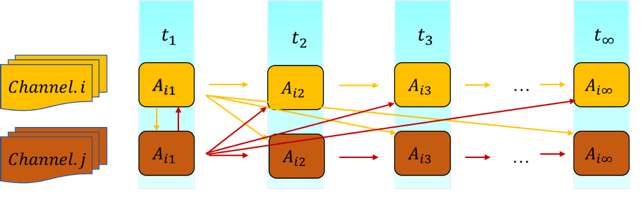
\includegraphics[width=0.8\textwidth]{2_ad_process}
\caption{广告在两个渠道上的生命周期}
\label{fig:2_ad_process}
\end{figure}

对于本渠道自身延迟的效果影响,我们可以使用强化学习中的累积折扣奖赏最大化处理;而对其他渠道产生的影响,我们通常要对全部的渠道进行建模,以捕捉到渠道之间的联系,但是,在广告投放的场景中,我们所能获得的数据非常少,如果使用仅有的少量数据对全部渠道进行建模,那么得到的模型自然时很差的。所以,一个自然的想法是,我们应该对每个渠道进行单独的建模,然后通过启发式的经验改进值函数的评估方法。

假设含有$n$个渠道的集合为$I=\{1,2,\cdots,n\}$,在某时刻,其他渠道$I\backslash\{i\}$对渠道$i$产生的影响记为$q_{i}^{'}$,定义为:
\begin{equation}\label{seq_ad_influence}
\begin{aligned}
q_{i}^{'}=\sum_{j\in I \backslash \{i\}} \sum_{k=0}^{\infty} \tau_{j,i,t+k+1} \cdot \gamma_{i}^{k} \cdot r_{j,t+k+1},\\
\tau_{j,i,t+k+1}=d \cdot \frac{c_{j,t+k+1}}{c_{i,t+k+1}},d<1.
\end{aligned}
\end{equation}

式$\eqref{seq_ad_influence}$中,$\gamma_{i}$表示渠道$i$的折扣因子,$\tau_{j,i,t+k+1}$是一个常数$d$乘以$t+k+1$时刻在第$j$个渠道上的花费与在第$i$个渠道上花费之比,$r_{j,t+k+1}$表示渠道$j$在$t+k+1$时刻所获的即时利润。从公式中可以看出,$\sum_{k=0}^{\infty} \gamma_{i}^{k} \cdot r_{j,t+k+1}$是近似为其他某一渠道获得的所获的累积利润,$\tau_{j,i,t+k+1}$通过某时刻第$j$个渠道上的花费与第$i$个渠道上花费的比值来反映渠道$j$对渠道$i$的投放效果的影响。

于是,考虑$q_{i}^{'}$并结合公式\eqref{seq2_qsa},可以得到改进的渠道$i$最优值函数的公式:
\begin{equation}
\label{seq_modified_q}
\begin{aligned}
q_{i}(S_{t},A_{t})&=\mathbb{E}[\sum_{k=0}^{\infty} \gamma_{i}^{k} r_{i,r+k+1} + \sum_{j \in I \backslash \{i\}} \sum_{k=0}^{\infty} \tau_{j,i,t+k+1} \cdot \gamma_{i}^{k} r_{j,t+k+1} | S_{t}=s, A_t = a]\\
&=\mathbb{E}[r_{i,t+1} + \gamma_{i} \sum_{k=0}^{\infty} \gamma_{i}^{k} r_{r+k+2} + \sum_{j \in \backslash \{i\}} \tau_{j,i,t+1}r_{j, t+1} \\
&+ \gamma_{i} \sum_{j \in \backslash \{i\}} \sum_{k=0}^{\infty} \tau_{j,i,t+k+2} \cdot \gamma_{i}^{k} r_{j,t+k+2} | S_{t}=s, A_t = a]\\
&=\mathbb{E}[r_{i,t+1} + \sum_{j \in I \backslash \{i\}} \tau_{j,i,t+1} r_{j, t+1} + \gamma_{i} q_{i}(S_{t+1},A_{t+1}) | S_{t}=s, A_t = a]\\
\end{aligned}
\end{equation}


因此,我们就可以将$t$时刻渠道$i$的Q值迭代的更新公式改为:
% \begin{equation}
% \begin{aligned}
\begin{dmath}
\label{seq_modified_Q}
Q_{i}(S_{t},A_{t})=Q_{i}(S_{t},A_{t})+\alpha_{i}(r_{i, t+1} + \sum_{j \in I \backslash \{i\}} \tau_{j,i,t+1} r_{j, t+1} + \gamma_{i} max_{a_{'}} Q_{i}(S_{t+1}, a^{'}) - Q_{i}(S_{t},A_{t}))
% \end{aligned}
% \end{equation}
\end{dmath}

\subsection{改进的探索方法}
在传统的Q-learning学习方法中,我们通常采用的ε-greedy的探索方法。其思想为:以概率$\epsilon$随机选择一个行为,以(1-$\epsilon$)的概率选择最优的策略。 $\epsilon-greedy$平衡了利用(exploitation)和探索(exploration),其中选取动作值函数最大的部分为利用,其他非最优动作仍有概率为探索部分。但是这种方法存在两个弱点:第一,它只关心从行为中得到了多少奖赏,而不知道它对该行为了解多少,即所有行为在任何时候都是平等的。所以,即使某一行为在初试经历中没有获得奖赏,它仍然有会被探索到。第二,因为采用随机抽样的方法,所以很容易被负面的经历所干扰。因此,特别是在小数据集的情况下,$\epsilon-greedy$的探索方法是不完全适用于广告投放的场景中。所以,我们在探索中,我们要不仅考虑到我们对该行为的了解程度,而且要减少随机采样的操作。所以,我们可以使用如下方式来选择行为:
\begin{equation}
\begin{aligned}
\argmax_{a}[Q(s,a)+\varphi \sqrt{\frac{ln n^{'}}{n_{a}^{'}}}]
\end{aligned}
\end{equation}
其中,$n^{'}$表示所有行为被选择的次数,$n_{a}^{'}$表示行为$a$被选择的次数,常数$\varphi > 0$控制了探索的程度。

因此,$t$时刻渠道$i$的Q值迭代的更新公式改为:

\begin{dmath}
\label{seq_modified_Q_}
Q_{i}(S_{t},A_{t})=Q_{i}(S_{t},A_{t})+\alpha_{i}(r_{i, t+1} + \sum_{j \in I \backslash \{i\}} \tau_{j,i,t+1} r_{j, t+1} + \gamma_{i} \max_{a_{'}} Q_{i}(S_{t+1}, \argmax_{a^{'}}[Q(S_{t},A_{t})+ \varphi_{i} \sqrt{\frac{ln n_{i}^{'}}{n^{'}_{i a^{'}}}}]) - Q_{i}(S_{t},A_{t}))
\end{dmath}



\subsection{批处理以及整体架构}
经过上述改进Q值函数的迭代公式以及探索方法后,对SVR+Q+MCKP分块模型的流程也要做相应的改进。因为在更新Q值函数时,需要考到到其他渠道的影响,这就要求我们应该利用同一时刻的投放数据同时对所有渠道进行更新。同时,为了使训练过程更加符合真是的投放场景,参考文献\citep{pednault2002sequential}采取了批强化学习的训练方法。改进后的模型伪代码如算法\eqref{algo:RBF-SVR+Q_final}和算法\eqref{algo:RBF-SVR+Q_2}所示。

\begin{algorithm}[htbp]
\small
\SetAlgoLined
\SetKwRepeat{Repeat}{repeat}{until} 
\SetKwData{Left}{left}\SetKwData{This}{this}\SetKwData{Up}{up}

输入:全部渠道的集合$I=\{1,2,\cdots,n\}$,$n$为渠道的总数;全部渠道的投放数据$O=\{O_{1},O_{2},\cdots,O_{n}\}$,其中$O_{i}=\{<\mathbf{s}_{i,t},c_{i,t},r_{i,t+1},\mathbf{s}_{i,t+1}>|t=1,\cdots,N_{i}\}$表示第$i$个渠道的数据集,$N_{i}$表示第$i$个渠道的数据量;Q函数的学习率$\alpha_{i}$,折扣因子$\gamma_{i}$,$i=1,2,\cdots,n$,最大迭代次数$P$,SVR+Q模型中的正则化参数$C$,RBF核函数的宽度$\sigma$\;

\For{$i=1$ \KwTo $n$}{
	利用算法$\ref{algo:DC}$求出渠道$i$的离散区间$\bm{\omega}_{i}=\{\omega_{i,1},\omega_{i,2},\cdots,\omega_{i,M_{i}+1}\}$,$M_{i}$表示第$i$个渠道形成的离散区间的个数\;
	将每个区间样本的平均花费值作为该区间所对应的行为值$a$,并且将此行为值添加到该区间的每个样本中,样本格式变为:$<\mathbf{s}_{i,t},c_{i,t},a_{i,t},r_{i,t+1},\mathbf{s}_{i,t+1}>$ \;
	按照行为值的不同,建立为$M_{i}$个样本单元$D_{i,h}$,$h=\{1,\cdots,M_{i}\}$,且此时,$D_{i,h}=\varnothing$ \;
}

数据转换:将全部渠道的数据$O$划分成$K$个情节$e$,即:$O=\{e_{k}|k=1,\cdots,K\}$,每个情节$e_{k}$包括$l_{k}$天的投放数据,即:$e_{k}=\{O^{'}_{j}|j=1,\cdots,l_{k}\}$,每一天的投放数据$O^{'}_{j}$又由$n$个渠道组成,即:$O^{'}_{j}=\{<\mathbf{s}_{k,j,i},c_{k,j,i},a_{k,j,i},r_{k,j+1,i},\mathbf{s}_{k,j+1,i}>|i=1,\cdots,n\}$\;

% 新增输入数据:SVR+Q模型中的正则化参数$C_{i,j}$,RBF核函数的宽度$\sigma_{i,j}$,,其中$i=1,2,\cdots,n$表示渠道号,$j=1,2,\cdots,M_{i}$表示渠道所对应的离散行为个数\;

\For{$k = 1$ \KwTo $K$}{
	\For{$j = 1$ \KwTo $l_{k}$}{
		\For{$i = 1$ \KwTo $n$}{
			按照算法\eqref{algo:RBF-SVR+Q_2}第10行的公式,计算样本的Q值,并将Q值添加到该样本中,其格式变为:$<\mathbf{s}_{k,j,i},c_{k,j,i},a_{k,j,i},r_{k,j+1,i},Q^{(0)}_{k,j,i}(\mathbf{s}_{k,j,i}),\mathbf{s}_{k,j+1,i}>$\;
			将该样本按照行为值分流到对应的样本单元中$D_{i,h}$,$h=\{1,\cdots,M_{i}\}$\;
		}
	}
}
$p=0$\;
\Repeat{$p=P$}{
	SVR+Q分块多路逼近迭代过程(算法$\ref{algo:RBF-SVR+Q_2}$)\;
	$p=p+1$ \;
}
输出各渠道的最终的Q值函数:$\text{Q}_{i}^{(P)}=\cup_{j=1,\cdots,l_{i}}\text{Q}_{i,j}^{(P)}$\; 
全渠道的Q值函数:$\text{Q}={\text{Q}_{i}^{(P)}}$,$i=1,\cdots,n$\;
$Res = MCKP(B,\text{Q})$\;
输出:最终的分配策略$Res$\;
\caption{SVR+Q+MCKP算法}
\label{algo:RBF-SVR+Q_final}
\end{algorithm}

\begin{algorithm}[htbp]
\small
\SetAlgoLined
\SetKwRepeat{Repeat}{repeat}{until} 
	\For{$i=1$ \KwTo $n$}{
		\For{$j=1$ \KwTo $M_{i}$}{
			对每个样本单元$D_{i,j}$,利用SVR+Q分块逼近模型进行回归建模,得到当前轮的Q值函数分块模型:$\text{Q}_{i,j}^{p}=f_{i,j}^{(p)}(\bm{s})=\sum_{m=1}^{N_{i,j}}(\hat{\alpha}_{i,j,m}^{(p)}-\alpha_{i,j,m}^{(p)})k(\bm{s},\bm{s}_{i,j,m})+b_{i,j}^{(p)}$,$N_{i,j}$表示第$i$个渠道的第$j$个样本空间中样本的个数\;
		}
	}

	\For{$k = 1$ \KwTo $K$}{
		\For{$j = 1$ \KwTo $l_{k}$}{
			\For{$i=1$ \KwTo $n$}{
				更新Q值函数:\\
				$\text{Q}_{k,j+1,i}^{(p+1)} = \text{Q}_{k,j+1,i}^{(p)} + \alpha_{i}^{(p)} (r_{k,j+1,i}+\gamma_{i} \argmax_{a^{'}}[f_{i,ID(a_{i}^{'})}^{(p)}(\bm{s}_{k,j+1,i})+\varphi_{i} \sqrt{\frac{ln n_{i}^{'}}{n_{i,ID(a_{i}^{'})}^{'}}}]) - \text{Q}_{k,j+1,i}^{(p)}$\;
				$ID(a_{i}^{'})$第$i$个渠道行为$a_{i}^{'}$所对应的编号,$n_{i}^{'}$ 为第$i$个渠道所有行为已经选择的次数,$n_{i,ID(a_{i}^{'})}^{'}$表示行为$ID(a_{i}^{'})$被选择的次数\;
				}
				利用上式更新在样本单元中的Q值\;
			}
		}

\caption{SVR+Q分块逼近的迭代过程}
\label{algo:RBF-SVR+Q_2}
\end{algorithm}


\section{本章小结}
在本章中,首先分析了在直复营销体系下,基于广告代理商的投放预算分配问题,并说明了将全渠道的LTV作为评价广告投放效果的指标,以此作为选择强化学习解决该问题的出发点。另外,又分析在应用时所面临的场景复杂、数据量少以及预算约束等问题。然后,在小数据集下,针对值函数逼近问题提出了SVR+Q多路逼近模型,加快收敛速度的同时提高手链精度,并将SVR+Q与MCKP结合,应用于多渠道资金分配问题。最后,提出一个花费空间离散化的方法,以更好的应用SVR+Q+MCKP模型、针对多渠道之间的影响提出一种改进值函数的估计方法,而且提出了一个在小数据集下高效的探索方法。



\chapter{仿真实验}

\section{直销营销仿真分析}
\subsection{数据集介绍}
\subsection{仿真环境构建}
\subsection{仿真结果及分析}

\section{广告投放仿真分析}
\subsection{数据集介绍}
\subsection{仿真环境构建}
\subsection{仿真结果及分析}

\section{本章小结}

 
\chapter{结论}


\section{工作总结}

\section{工作展望}
 
% \chapter{数学}

\section{数学符号}

模板定义了一些正体(upright)的数学符号:
\begin{center}
\begin{tabular}{rl}
  \toprule
    符号                 & 命令 \\
  \midrule
    常数$\eu$     & \verb|\eu| \\
    复数单位$\iu$ & \verb|\iu| \\
    微分符号$\diff$ & \verb|\diff| \\
    $\argmax$         & \verb|\argmax| \\
    $\argmin$         & \verb|\argmin| \\
  \bottomrule
\end{tabular}
\end{center}

更多的例子:
\begin{equation}
  \eu^{\iu\pi} + 1 = 0
\end{equation}
\begin{equation}
  \frac{\diff^2u}{\diff t^2} = \int f(x) \diff x
\end{equation}
\begin{equation}
  \argmin_x f(x)
\end{equation}

\section{定理、引理和证明}

\begin{definition}
    If the integral of function $f$ is measurable and non-negative, we define
    its (extended) \textbf{Lebesgue integral} by
    \begin{equation}
        \int f = \sup_g \int g,
    \end{equation}
    where the supremum is taken over all measurable functions $g$ such that
    $0 \leq g \leq f$, and where $g$ is bounded and supported on a set of
    finite measure.
\end{definition}

\begin{example}
    Simple examples of functions on $\mathbb{R}^d$ that are integrable
    (or non-integrable) are given by
    \begin{equation}
        f_a(x) =
        \begin{cases}
            |x|^{-a} & \text{if } |x| \leq 1,\\
            0 & \text{if } x > 1.
        \end{cases}
    \end{equation}
    \begin{equation}
        F_a(x) = \frac{1}{1 + |x|^a}, \qquad \text{all } x \in \mathbb{R}^d.
    \end{equation}
    Then $f_a$ is integrable exactly when $a < d$, while $F_a$ is integrable
    exactly when $a > d$.
\end{example}

\begin{lemma}[Fatou]
    Suppose $\{f_n\}$ is a sequence of measurable functions with $f_n \geq 0$.
    If $\lim_{n \to \infty} f_n(x) = f(x)$ for a.e. $x$, then
    \begin{equation}
        \int f \leq \liminf_{n \to \infty} \int f_n.
    \end{equation}
\end{lemma}

\begin{remark}
    We do not exclude the cases $\int f = \infty$,
    or $\liminf_{n \to \infty} f_n = \infty$.
\end{remark}

\begin{corollary}
    Suppose $f$ is a non-negative measurable function, and $\{f_n\}$ a sequence
    of non-negative measurable functions with
    $f_n(x) \leq f(x)$ and $f_n(x) \to f(x)$ for almost every $x$. Then
    \begin{equation}
        \lim_{n \to \infty} \int f_n = \int f.
    \end{equation}
\end{corollary}

\begin{proposition}
    Suppose $f$ is integrable on $\mathbb{R}^d$. Then for every $\epsilon > 0$:
    \begin{enumerate}
        \renewcommand{\theenumi}{\roman{enumi}}
        \item There exists a set of finite measure $B$ (a ball, for example) such that
        \begin{equation}
            \int_{B^c} |f| < \epsilon.
        \end{equation}
        \item There is a $\delta > 0$ such that
        \begin{equation}
            \int_E |f| < \epsilon \qquad \text{whenever } m(E) < \delta.
        \end{equation}
    \end{enumerate}
\end{proposition}

\begin{theorem}
    Suppose $\{f_n\}$ is a sequence of measurable functions such that
    $f_n(x) \to f(x)$ a.e. $x$, as $n$ tends to infinity.
    If $|f_n(x)| \leq g(x)$, where $g$ is integrable, then
    \begin{equation}
        \int |f_n - f| \to 0 \qquad \text{as } n \to \infty,
    \end{equation}
    and consequently
    \begin{equation}
        \int f_n \to \int f \qquad \text{as } n \to \infty.
    \end{equation}
\end{theorem}

\begin{proof}
    Trivial.
\end{proof}



\section{自定义}

\newtheorem*{axiomofchoice}{Axiom of choice}
\begin{axiomofchoice}
    Suppose $E$ is a set and ${E_\alpha}$ is a collection of
    non-empty subsets of $E$. Then there is a function $\alpha
    \mapsto x_\alpha$ (a ``choice function'') such that
    \begin{equation}
        x_\alpha \in E_\alpha,\qquad \text{for all }\alpha.
    \end{equation}
\end{axiomofchoice}

\newtheorem{observation}{Observation}
\begin{observation}
    Suppose a partially ordered set $P$ has the property
    that every chain has an upper bound in $P$. Then the
    set $P$ contains at least one maximal element.
\end{observation}
\begin{proof}[A concise proof]
    Obvious.
\end{proof}

% \chapter{浮动体}

\section{三线表}

三线表是《撰写手册》推荐使用的方式,如表~\ref{tab:exampletable}。
\begin{table}[htbp]
  \centering
  \caption{这里是表的标题}
  \label{tab:exampletable}
  \begin{tabular}{cl}
    \toprule
      操作系统 & TeX 发行版 \\
    \midrule
      所有 & TeX Live \\
      macOS & MacTeX \\
      Windows & MikTeX \\
    \bottomrule
  \end{tabular}
  \note{一个很长长长长长长长长长长长长长长长长长长长长长长长长长长长长长长长长长
  长长长长长长长长长长长的表注。}
\end{table}



\section{长表格}

超过一页的表格要使用专门的 \texttt{longtable} 环境(表~\ref{tab:longtable})。
\begin{longtable}{ccc}
  % 首页表头
  \caption[长表格演示]{长表格演示}
  \label{tab:longtable}\\
  \toprule[1.5pt]
    名称  & 说明 & 备注\\
  \midrule[1pt]
  \endfirsthead
  % 续页表头
  \caption[]{长表格演示(续)} \\
  \toprule[1.5pt]
  名称  & 说明 & 备注 \\
  \midrule[1pt]
  \endhead
  % 首页表尾
  \hline
  \multicolumn{3}{r}{\small 续下页}
  \endfoot
  % 续页表尾
  \bottomrule[1.5pt]
  \endlastfoot

  AAAAAAAAAAAA   &   BBBBBBBBBBB   &   CCCCCCCCCCCCCC   \\
  AAAAAAAAAAAA   &   BBBBBBBBBBB   &   CCCCCCCCCCCCCC   \\
  AAAAAAAAAAAA   &   BBBBBBBBBBB   &   CCCCCCCCCCCCCC   \\
  AAAAAAAAAAAA   &   BBBBBBBBBBB   &   CCCCCCCCCCCCCC   \\
  AAAAAAAAAAAA   &   BBBBBBBBBBB   &   CCCCCCCCCCCCCC   \\
  AAAAAAAAAAAA   &   BBBBBBBBBBB   &   CCCCCCCCCCCCCC   \\
  AAAAAAAAAAAA   &   BBBBBBBBBBB   &   CCCCCCCCCCCCCC   \\
  AAAAAAAAAAAA   &   BBBBBBBBBBB   &   CCCCCCCCCCCCCC   \\
  AAAAAAAAAAAA   &   BBBBBBBBBBB   &   CCCCCCCCCCCCCC   \\
  AAAAAAAAAAAA   &   BBBBBBBBBBB   &   CCCCCCCCCCCCCC   \\
  AAAAAAAAAAAA   &   BBBBBBBBBBB   &   CCCCCCCCCCCCCC   \\
  AAAAAAAAAAAA   &   BBBBBBBBBBB   &   CCCCCCCCCCCCCC   \\
  AAAAAAAAAAAA   &   BBBBBBBBBBB   &   CCCCCCCCCCCCCC   \\
  AAAAAAAAAAAA   &   BBBBBBBBBBB   &   CCCCCCCCCCCCCC   \\
  AAAAAAAAAAAA   &   BBBBBBBBBBB   &   CCCCCCCCCCCCCC   \\
  AAAAAAAAAAAA   &   BBBBBBBBBBB   &   CCCCCCCCCCCCCC   \\
  AAAAAAAAAAAA   &   BBBBBBBBBBB   &   CCCCCCCCCCCCCC   \\
  AAAAAAAAAAAA   &   BBBBBBBBBBB   &   CCCCCCCCCCCCCC   \\
  AAAAAAAAAAAA   &   BBBBBBBBBBB   &   CCCCCCCCCCCCCC   \\
  AAAAAAAAAAAA   &   BBBBBBBBBBB   &   CCCCCCCCCCCCCC   \\
\end{longtable}



\section{插图}

有的同学可能习惯了“下图”、“上表”这样的相对位置引述方式,希望浮动体放在固定位置。
事实上,这是不合理的,因为这很容易导致大片的空白。
在科技论文中,标准的方式是“图\ref{fig:logo}”、“表~\ref{tab:exampletable}”这样的
因数方式。
\begin{figure}[htbp]
\centering

\includegraphics[width=.3\textwidth]{ustc_logo_fig}
\caption{测试图片}
\label{fig:logo}
\end{figure}

关于更多的插图方式,\href{https://arxiv.org}{arXiv} 上的大部分文献会提供 \TeX{}
源码,大家可以参考学习。



\section{算法环境}

模板中使用 \texttt{algorithm2e} 宏包实现算法环境。关于该宏包的具体用法,
请阅读宏包的官方文档。

\begin{algorithm}[htbp]
\small
\SetAlgoLined
\KwData{this text}
\KwResult{how to write algorithm with \LaTeX2e }

initialization\;
\While{not at end of this document}{
    read current\;
    \eIf{understand}{
        go to next section\;
        current section becomes this one\;
    }{
        go back to the beginning of current section\;
    }
}
\caption{算法示例1}
\label{algo:algorithm1}
\end{algorithm}

注意,我们可以在论文中插入算法,但是插入大段的代码是愚蠢的。
然而这并不妨碍有的同学选择这么做,对于这些同学,建议用 \textsf{listings} 宏包。

% \chapter{引用文献标注方法}

\section{顺序编码制}

\subsection{角标数字标注法}

\citestyle{super}
\noindent
\begin{tabular}{l@{\quad$\Rightarrow$\quad}l}
  \verb|\cite{knuth86a}| & \cite{knuth86a}\\
  \verb|\citet{knuth86a}| & \citet{knuth86a}\\
  \verb|\citet[chap.~2]{knuth86a}| & \citet[chap.~2]{knuth86a}\\[0.5ex]
  \verb|\citep{knuth86a}| & \citep{knuth86a}\\
  \verb|\citep[chap.~2]{knuth86a}| & \citep[chap.~2]{knuth86a}\\
  \verb|\citep[see][]{knuth86a}| & \citep[see][]{knuth86a}\\
  \verb|\citep[see][chap.~2]{knuth86a}| & \citep[see][chap.~2]{knuth86a}\\[0.5ex]
  \verb|\citet*{knuth86a}| & \citet*{knuth86a}\\
  \verb|\citep*{knuth86a}| & \citep*{knuth86a}\\
\end{tabular}
\par\noindent
\begin{tabular}{l@{\quad$\Rightarrow$\quad}l}
  \verb|\citet{knuth86a,tlc2}| & \citet{knuth86a,tlc2}\\
  \verb|\citep{knuth86a,tlc2}| & \citep{knuth86a,tlc2}\\
  \verb|\cite{knuth86a,knuth84}| & \cite{knuth86a,knuth84}\\
  \verb|\citet{knuth86a,knuth84}| & \citet{knuth86a,knuth84}\\
  \verb|\citep{knuth86a,knuth84}| & \citep{knuth86a,knuth84}\\
  \verb|\cite{knuth86a,knuth84,tlc2}| & \cite{knuth86a,knuth84,tlc2}\\
\end{tabular}



\subsection{数字标注法}

\citestyle{numbers}
\noindent
\begin{tabular}{l@{\quad$\Rightarrow$\quad}l}
  \verb|\cite{knuth86a}| & \cite{knuth86a}\\
  \verb|\citet{knuth86a}| & \citet{knuth86a}\\
  \verb|\citet[chap.~2]{knuth86a}| & \citet[chap.~2]{knuth86a}\\[0.5ex]
  \verb|\citep{knuth86a}| & \citep{knuth86a}\\
  \verb|\citep[chap.~2]{knuth86a}| & \citep[chap.~2]{knuth86a}\\
  \verb|\citep[see][]{knuth86a}| & \citep[see][]{knuth86a}\\
  \verb|\citep[see][chap.~2]{knuth86a}| & \citep[see][chap.~2]{knuth86a}\\[0.5ex]
  \verb|\citet*{knuth86a}| & \citet*{knuth86a}\\
  \verb|\citep*{knuth86a}| & \citep*{knuth86a}\\
\end{tabular}
\par\noindent
\begin{tabular}{l@{\quad$\Rightarrow$\quad}l}
  \verb|\citet{knuth86a,tlc2}| & \citet{knuth86a,tlc2}\\
  \verb|\citep{knuth86a,tlc2}| & \citep{knuth86a,tlc2}\\
  \verb|\cite{knuth86a,knuth84}| & \cite{knuth86a,knuth84}\\
  \verb|\citet{knuth86a,knuth84}| & \citet{knuth86a,knuth84}\\
  \verb|\citep{knuth86a,knuth84}| & \citep{knuth86a,knuth84}\\
  \verb|\cite{knuth86a,knuth84,tlc2}| & \cite{knuth86a,knuth84,tlc2}\\
\end{tabular}



\section{著者-出版年制标注法}

\citestyle{authoryear}
\noindent
\begin{tabular}{l@{\quad$\Rightarrow$\quad}l}
  \verb|\cite{knuth86a}| & \cite{knuth86a}\\
  \verb|\citet{knuth86a}| & \citet{knuth86a}\\
  \verb|\citet[chap.~2]{knuth86a}| & \citet[chap.~2]{knuth86a}\\[0.5ex]
  \verb|\citep{knuth86a}| & \citep{knuth86a}\\
  \verb|\citep[chap.~2]{knuth86a}| & \citep[chap.~2]{knuth86a}\\
  \verb|\citep[see][]{knuth86a}| & \citep[see][]{knuth86a}\\
  \verb|\citep[see][chap.~2]{knuth86a}| & \citep[see][chap.~2]{knuth86a}\\[0.5ex]
  \verb|\citet*{knuth86a}| & \citet*{knuth86a}\\
  \verb|\citep*{knuth86a}| & \citep*{knuth86a}\\
\end{tabular}
\par\noindent
\begin{tabular}{l@{\quad$\Rightarrow$\quad}l}
  \verb|\citet{knuth86a,tlc2}| & \citet{knuth86a,tlc2}\\
  \verb|\citep{knuth86a,tlc2}| & \citep{knuth86a,tlc2}\\
  \verb|\cite{knuth86a,knuth84}| & \cite{knuth86a,knuth84}\\
  \verb|\citet{knuth86a,knuth84}| & \citet{knuth86a,knuth84}\\
  \verb|\citep{knuth86a,knuth84}| & \citep{knuth86a,knuth84}\\
\end{tabular}



\section{其他形式的标注}

\noindent
\begin{tabular}{l@{\quad$\Rightarrow$\quad}l}
  \verb|\citealt{tlc2}| & \citealt{tlc2}\\
  \verb|\citealt*{tlc2}| & \citealt*{tlc2}\\
  \verb|\citealp{tlc2}| & \citealp{tlc2}\\
  \verb|\citealp*{tlc2}| & \citealp*{tlc2}\\
  \verb|\citealp{tlc2,knuth86a}| & \citealp{tlc2,knuth86a}\\
  \verb|\citealp[pg.~32]{tlc2}| & \citealp[pg.~32]{tlc2}\\
  \verb|\citenum{tlc2}| & \citenum{tlc2}\\
  \verb|\citetext{priv.\ comm.}| & \citetext{priv.\ comm.}\\
\end{tabular}

\noindent
\begin{tabular}{l@{\quad$\Rightarrow$\quad}l}
  \verb|\citeauthor{tlc2}| & \citeauthor{tlc2}\\
  \verb|\citeauthor*{tlc2}| & \citeauthor*{tlc2}\\
  \verb|\citeyear{tlc2}| & \citeyear{tlc2}\\
  \verb|\citeyearpar{tlc2}| & \citeyearpar{tlc2}\\
\end{tabular}



\citestyle{super}
\nocite{*}

\bibliography{bib/ustc}

\appendix
\chapter{论文规范}

\backmatter
\begin{acknowledgements}

在研究学习期间,我有幸得到了三位老师的教导,
他们是:我的导师,中国科大XXX研究员,中科院X昆明动物所马老师以及美国犹他大学的XXX老师。
三位深厚的学术功底,严谨的工作态度和敏锐的科学洞察力使我受益良多。
衷心感谢他们多年来给予我的悉心教导和热情帮助。

感谢XXX老师在实验方面的指导以及教授的帮助。
科大的XXX同学和XXX同学参与了部分试验工作,在此深表谢意。

\end{acknowledgements}

\begin{publications}

\section*{已发表论文}

\begin{enumerate}
\item Wang X, \bm{\text{Li P}}, Wang L, et al. A novel genetic algorithm based on circles for larger-scale traveling salesman problem[C]//Robotics and Automation Sciences (ICRAS), 2017 International Conference on. IEEE, 2017: 189-194.
% \item A A A A A A A A A
% \item A A A A A A A A A
\end{enumerate}

\section*{待发表论文}

\begin{enumerate}
\item Wang X, \bm{\text{Li P}}, Ammar H, et al. A budget allocation algorithm for multi-channel marketing with Q-learning [C]//Pattern Recognition (ICPR), 2018 24rd International Conference on. IEEE.(已接收)
\item Wang X, \bm{\text{Li P}}, Ammar H, et al. A hybrid model of deep Reinforcement Learning for direct marketing [C] // Next Generation Data-driven Networks (NGDN), 2018 International Workshop on. IEEE.(已接收)
\end{enumerate}

\section*{参与的科研项目}
\begin{enumerate}
\item A A A A A A A A A
% \item A A A A A A A A A
% \item A A A A A A A A A
\end{enumerate}

\end{publications}


\end{document}